\documentclass{templateNote}
\usepackage{tcolorbox}
\usepackage{tabularx}
\usepackage{hyperref}
\usepackage{amsmath}
\usepackage{amssymb}
\usepackage{pdflscape}
\usepackage{xcolor}
\usepackage{tikz}
\usepackage{soul}
\usepackage{media9}
\usepackage{adjustbox}
\usepackage{pdfpages}
% \usepackage[spanish,es-noquoting]{babel}

\begin{document}

\imagenlogoU{img/logoNGMFormal_sinF.png}
\linklogoU{https://github.com/NicoGomezM} 
\imagenlogoD{img/LogoElNube.png} %TODO: No se ve el logo
\linklogoD{https://github.com/MarceloPazPezo}
\titulo{Unidad 1}
\asignatura{Sistemas de Información}
\autor{
    \indent
    Marcelo \textsc{Paz Pezo} \\
    Nicolás \textsc{Gómez Morgado}
}

\vDoc{1.0.0}
\portada
\margenes
\tableofcontents
\newpage

\section{Sistemas de Información}
\begin{itemize}
    \item \textbf{Sistema:} Conjunto de partes que interactúan entre sí, para lograr un objetivo en común.
\end{itemize}
\begin{figure}[H]
    \centering
    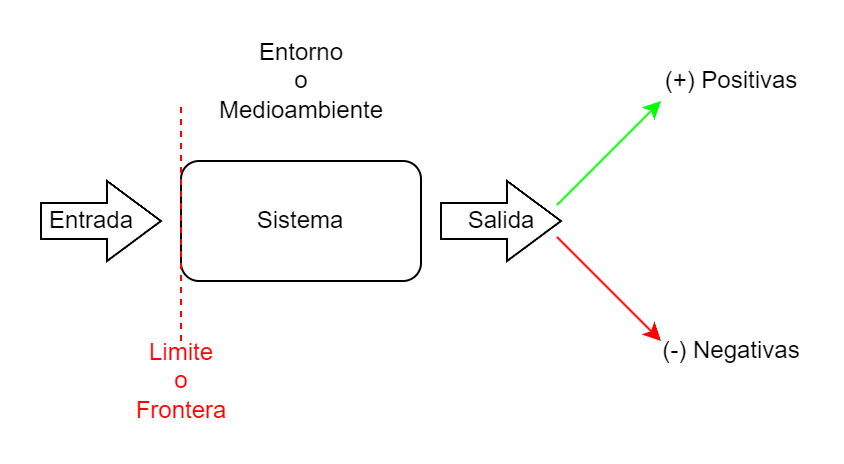
\includegraphics[width=0.9\textwidth]{img/diagrama Sistema.png}
\end{figure}

Definiciones:
\begin{itemize}
    \item \textbf{Entrada:} Todo aquello que el sistema recoge de su entorno para cumplir con su objetivo.
    \item \textbf{Salida:} Todo aquello que el sistema entrega al entorno producto del cumplimiento de su objetivo.
    
    Positivas (+) $\Rightarrow$  Sistema se beneficia
    
    Negativas (-) $\Rightarrow$ Sistema no se beneficia
    
    Salidas Positivas > $\space$ Salidas Negativas
\end{itemize}
\begin{itemize}
    \item \textbf{Sistema Abierto:} Es capaz de interactuar con el entorno por si solo.
    \item \textbf{Sistema Cerrado:} No es capaz de interactuar con el entorno por si solo.
    \item \textbf{Sinergia:} El todo es mas que las sumas de las partes. Las sumas de las partes cumplen un objetivo.
    \item \textbf{Conglomerado:} Conjunto de partes que no interactúan entre si.
    \item \textbf{Entropía:} Grado de desorden.
    \item \textbf{Dato:} Hecho conocido que no tiene valor.
    \item \textbf{Información:} Un dato al que se le agrega significado y utilidad.
    \item \textbf{Conocimiento Tácito:} Conocimiento que no se ve, como lo que esta en la mente de las personas.
    \item \textbf{Conocimiento Explícito:} Conocimiento que se puede ver, como textos o apuntes.
    \begin{itemize}
        \item Fácil de transmitir.
        \item Fácil de traspasar.
        \item Para transformar conocimiento tácito en explícito utilizando la documentación del conocimiento.
    \end{itemize}
    \item \textbf{Estrategia:} Es un camino a seguir para poder llegar al objetivo deseado.
    \item \textbf{Misión:} Razón de ser de la empresa.
    \item \textbf{Visión:} Sueño/Idea de llegar a ser.
    \item \textbf{Tecnologías de información:} Permiten desarrollar sistemas.
    \item \textbf{Recursos y capacidades:} El sistema no logra nada sin los recursos y capacidades.
    \item \textbf{Procesos:} Cosas que se hacen para convertir una entrada en salida.
    \item \textbf{Estructura:} Como se organiza.
    \item \textbf{Cultura:} Forma de hacer las cosas.
\end{itemize}

\begin{center}
    \begin{figure}[H]
        \centering
        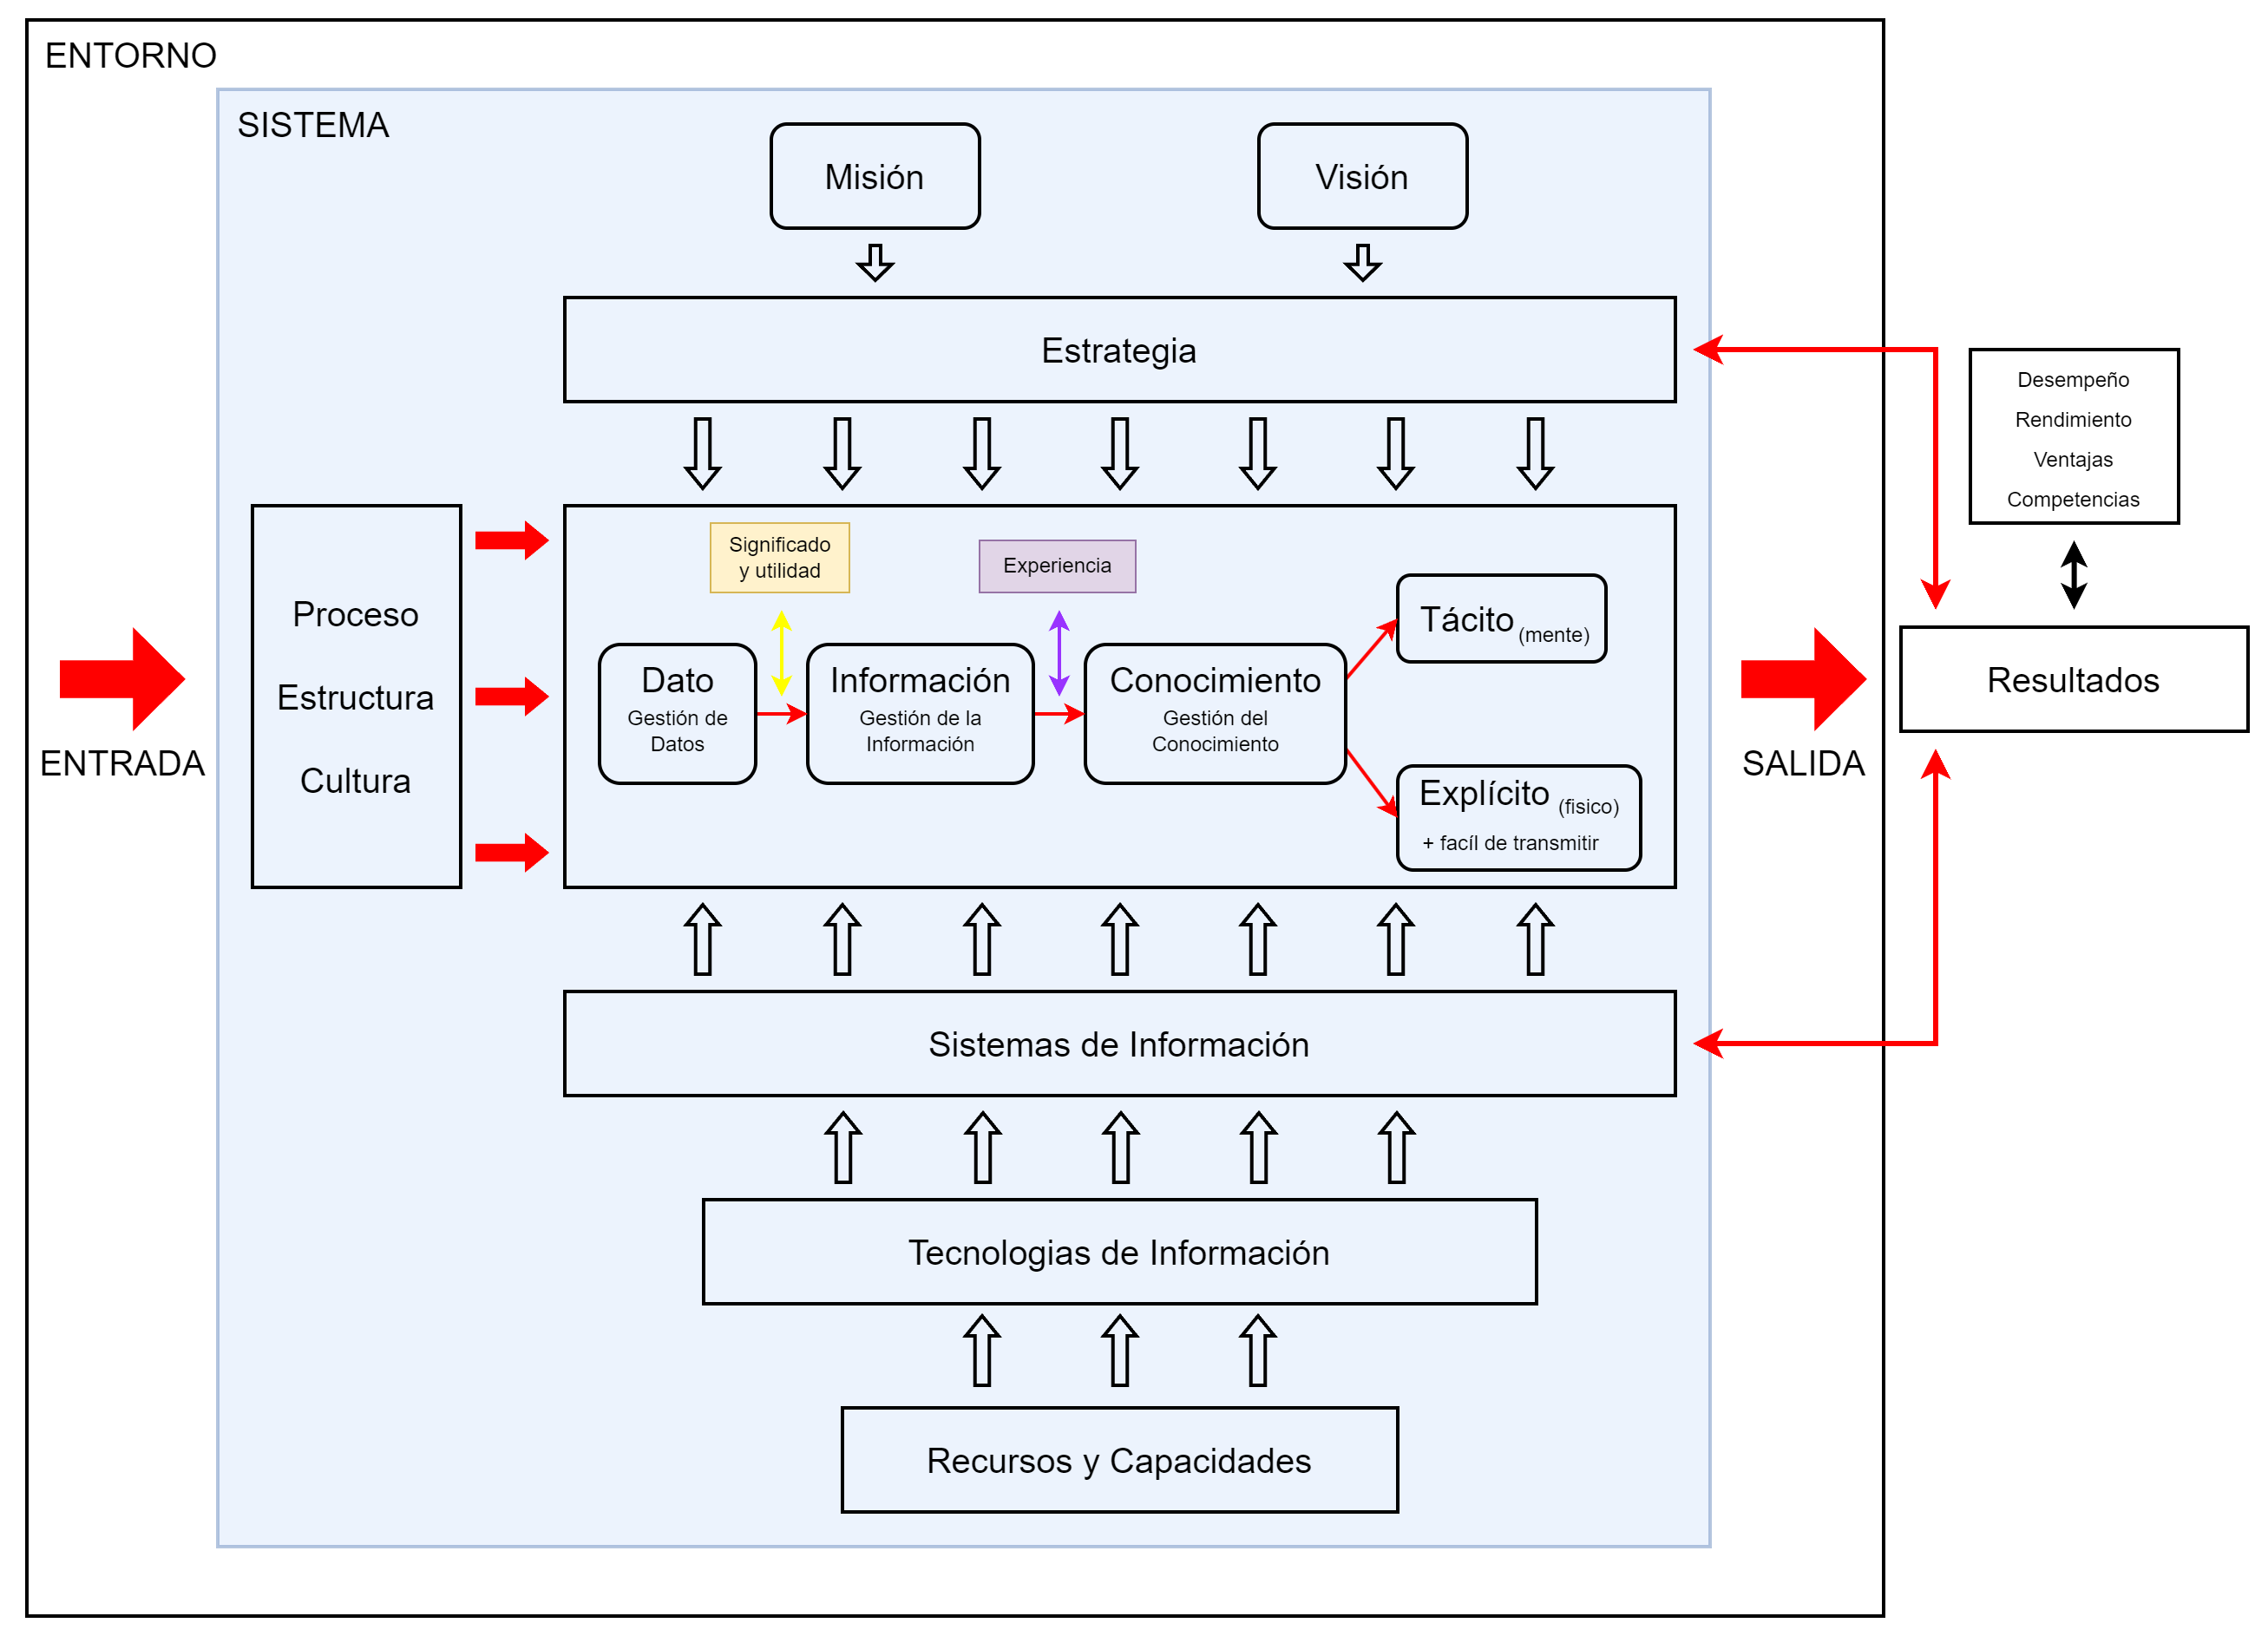
\includegraphics[width=1\textwidth]{img/digramaCompleto.png}
    \end{figure}
\end{center}

\section{Pirámide de Anthony}
\indent
Siempre encontramos 3 niveles:
\begin{figure}[H]
    \centering
    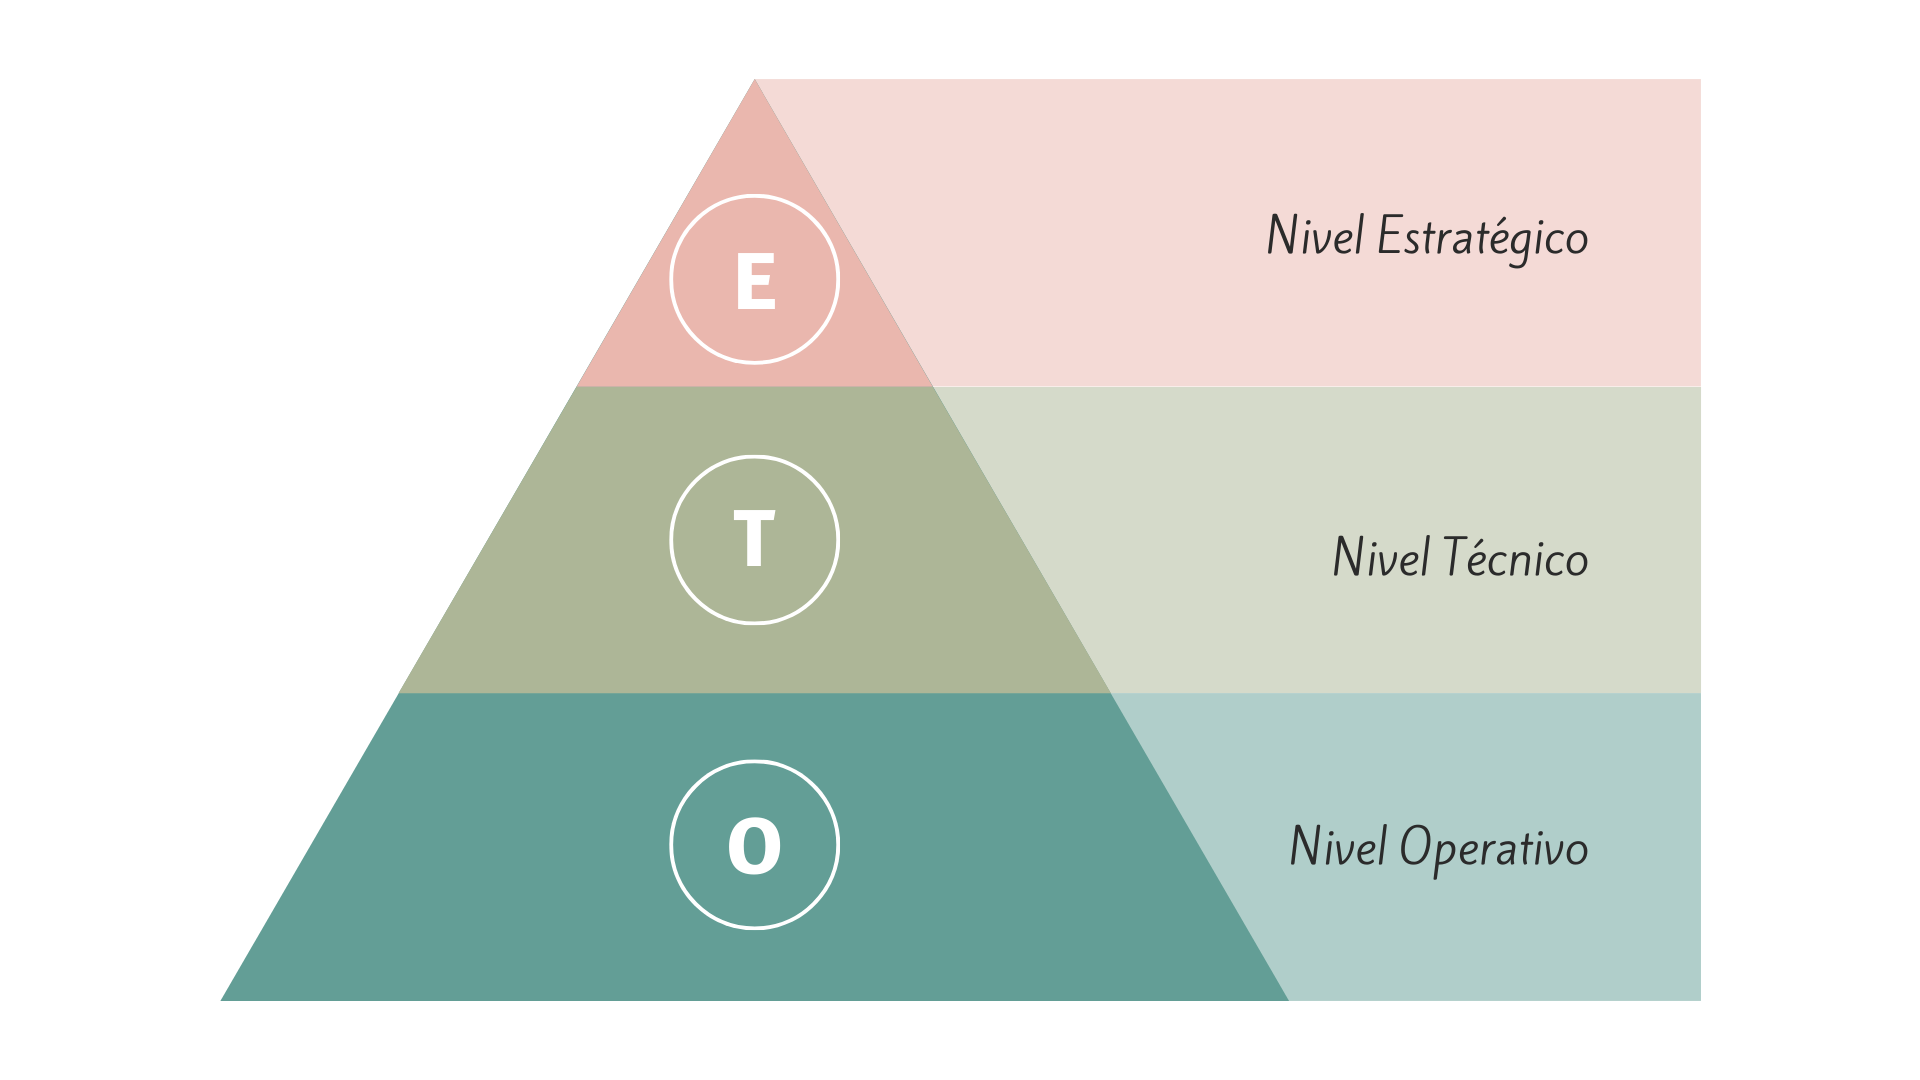
\includegraphics[width=0.7\textwidth]{img/PiramideAnthony.png}

\end{figure}
\begin{itemize}
    \item \textbf{Nivel Estratégico:} Definición de Misión; Largo Plazo.
    \item \textbf{Nivel Táctico:} Control de gestión; Mediano Plazo.
    \item \textbf{Nivel Operativo:} Actividades rutinarias; No cambian; Corto Plazo.
\end{itemize}
\textbf{Explicación:} La pirámide de Anthony. Ayuda a estructurar la información y/o las actividades de manera jerárquica. A menor nivel hay mas gente y las actividades son mas simples o rutinarias de hacer, y a mayor nivel hay menos personas y las decisiones son mas importantes por lo que hay un mayor plazo con el que se obtendrán los resultados.

\section{Características de la Información}
\begin{figure}[H]
    \begin{center}
        \noindent\adjustbox{center}{
            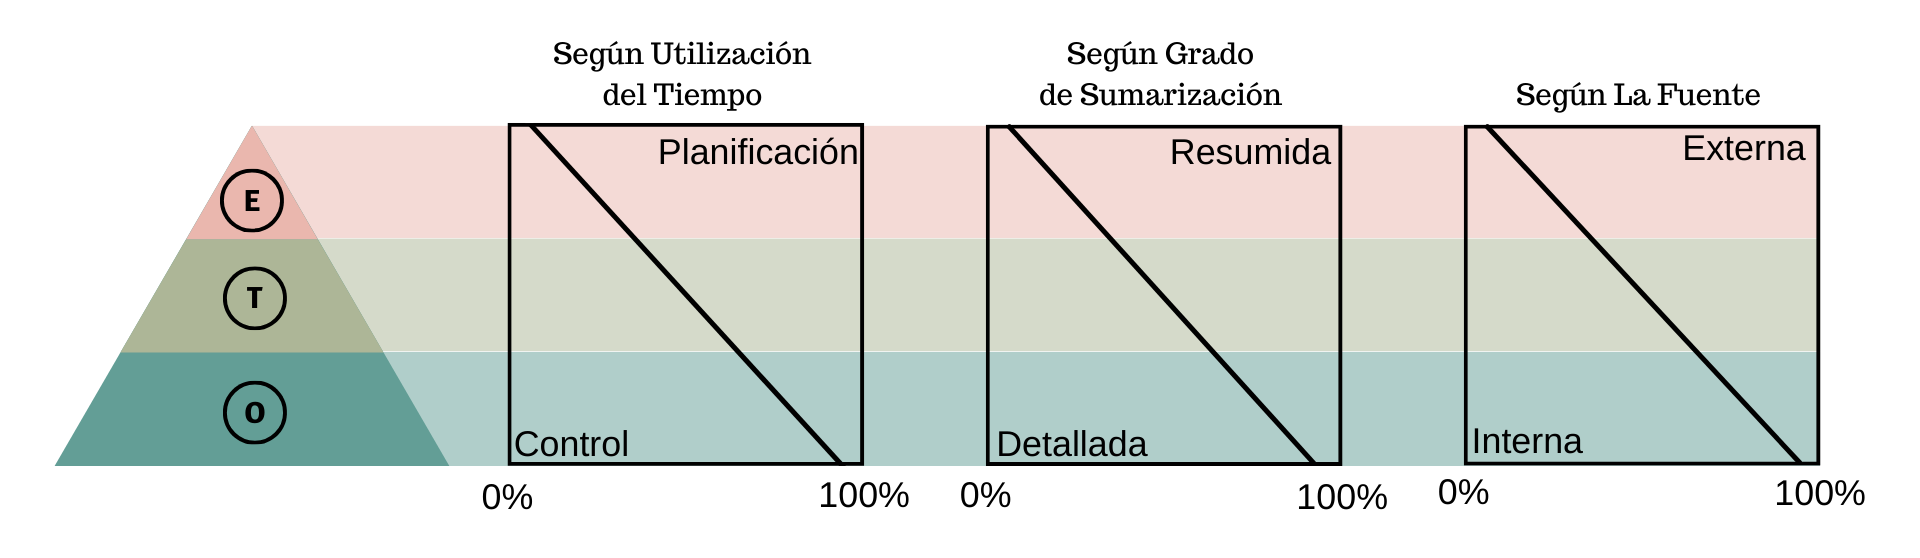
\includegraphics[width=1.2\textwidth]{img/PiramideAnthony2.png}
        }
    \end{center}
\end{figure}
\begin{itemize}
    \item \textbf{Según la utilización del tiempo:}
    \begin{itemize}
        \item La mayor parte del tiempo arriba se usa la información para planificación y abajo para tener un mayor control. Al no partir desde el 0 se dice que no hay un gran control sin planificación ni tampoco hay una gran planificación sin un mínimo de control.
        \item La información se utiliza la mayor cantidad del tiempo para actividades relacionadas con el control en el Operativo y mientras más se sube hay menor control y más planificación.
        \item * Entre más abajo sea el nivel la información se usará para actividades de mayor control y menor planificación. Entre más se suba en la pirámide la información se utilizara para planificación.
    \end{itemize}

    \item \textbf{Según el grado de sumarización:}
    \begin{itemize}
        \item Mientras mas abajo en niveles estemos la información será más detallada y entre más se suba será más resumida. Ejemplo: El gerente pide algo de una página o un pequeño gráfico, no un informe de 100 páginas.
    \end{itemize}

    \item \textbf{Según la fuente:}
    \begin{itemize}
        \item En niveles más bajos se pedirá información de fuentes internas para las actividades, entre más se suba será necesaria más de fuentes externas. Ejemplo: Una secretaria no tiene que saber sobre el dolar para la tarea que desempeña mientras que un gerente si.
    \end{itemize}
\end{itemize}

\begin{itemize}
    \item \textbf{Sistema de Información:} \hl{Conjunto formal de procesos} que operando sobre una \hl{colección de datos estructurados} recopila, elabora y distribuye (parte de) la información \hl{necesaria para la operación de dicha empresa} y para las actividades de \hl{dirección y control} correspondientes apoyando al menos en parte la toma de \hl{decisiones necesarias} para desempeñar las \hl{funciones y procesos} de acuerdo con la \hl{estrategia.}
    \begin{itemize}
        \item Un proceso es formal cuando esta bien definido, este proceso se puede estudiar.
        \item Un proceso es informal cuando no esta bien definido.
        \item Los datos están estructurados según la necesidad de la empresa.
        \item Recopilación, elaboración y distribución $\rightarrow$ Sistema con entrada, proceso y salida.
    \end{itemize}

    \item \textbf{Planificación de recursos empresariales (E.R.P):} Es la planificación de recursos empresariales por la traducción al español. Son una clasificación de software que esta hecho de una forma dividida en módulos e integra las diferentes partes para mejorar la eficiencia. Son muy caros, son difíciles de implementar si se seguía un sistema previo con cierta cultura.

    \item \textbf{Plan informático:} Estrategias de sistemas y tecnologías de información.
\end{itemize}

\section{Curva de Nolan}
\begin{figure}[H]
    \centering
    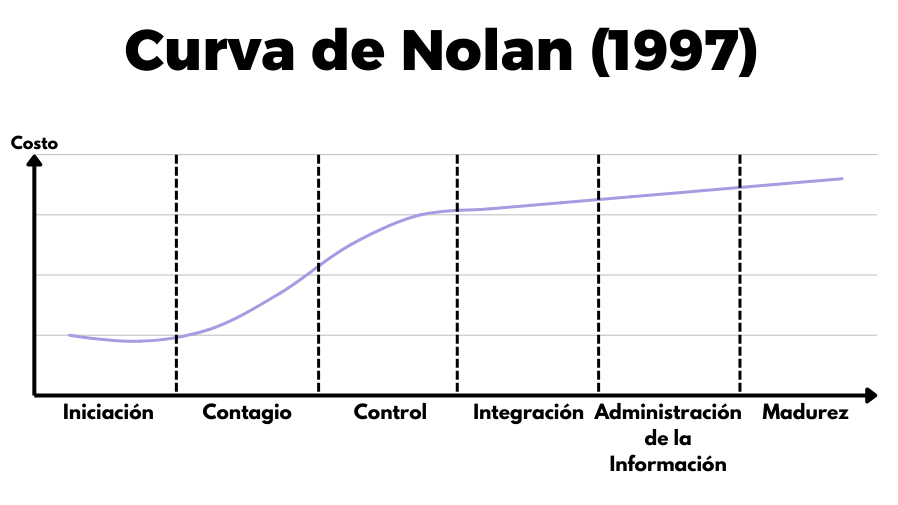
\includegraphics[width=0.7\textwidth]{img/CurvaDeNolan.png}
\end{figure}
\noindent Es una curva hecha en los años 1979 por Nolan y un amigo tratando originalmente mostrar como evolucionaba el costo en el tiempo. Actualmente, o para este ramo la usamos para observar como evolucionan los sistemas de información.    
\begin{itemize}
    \item \textbf{Inicialización:} Se empiezan a usar los primeros computadores, la gente que usaba estas maquinas eran vistos como raros y existían pocos usándolas.
    
    \item \textbf{Contagio:} Se dan cuenta que la gente que utiliza estos sistemas y tecnologías les beneficia y mejora la eficacia del trabajo. Todos empiezan a compra computadores por lo mismo.
    
    \item \textbf{Control:} Llega un momento en que los computadores, sistemas y tecnologías están llegando a muchas personas y sin control por lo que se reduce su venta quedando solo para un grupo selecto.
    
    \item \textbf{Integración:} Se empieza a integrar de mejor manera los sistemas a las empresas para que exista comunicación entre areas y mejore la eficacia.
    
    \item \textbf{Administración de la información:} Los sistemas y la información son algo importante de la organización por lo que se le empieza a tomar más en serio considerándolos como recursos administrables.
    
    \item \textbf{Madurez:} No hay miedo a las tecnologías o sistemas.
\end{itemize}
\begin{center}
    \textit{Planificación $\rightarrow$ Organización $\rightarrow$ Dirección $\rightarrow$ Control}
    \begin{figure}[H]
        \centering
        \vspace*{\fill}
        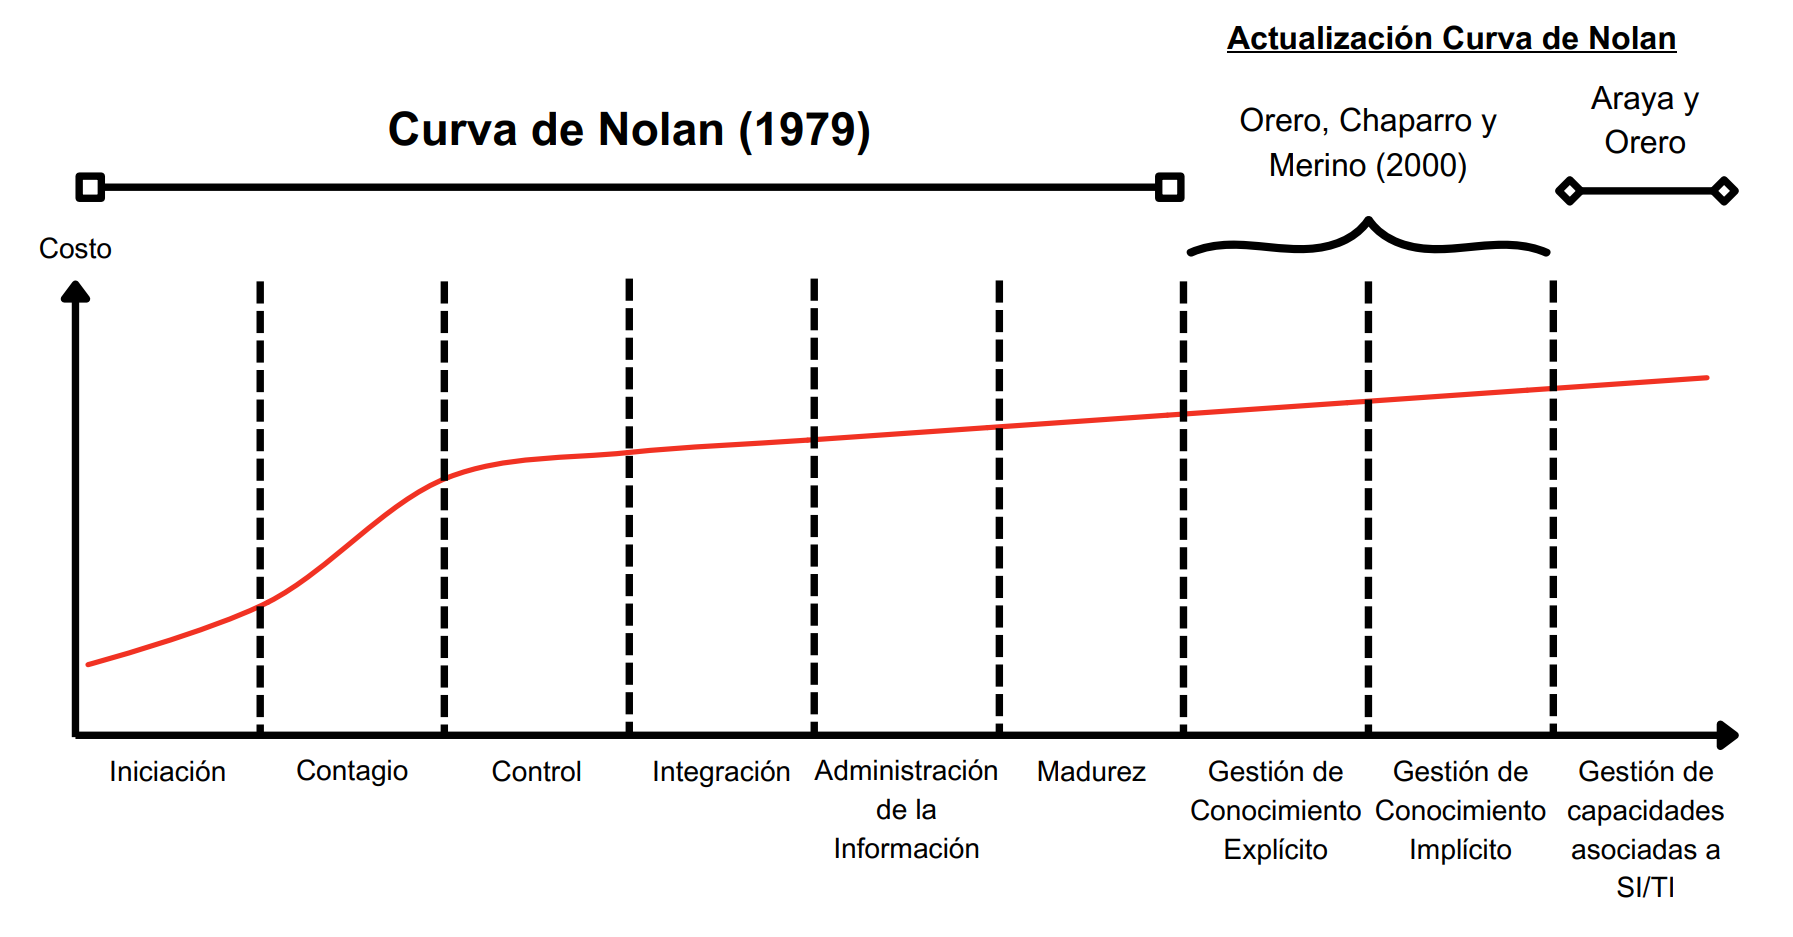
\includegraphics[width=1\textwidth,height=0.30\textheight,keepaspectratio]{img/CurvaDeNolanActualizada.png}
        \vspace*{\fill}
    \end{figure}
\end{center}
% \includepdf[pages={8,9}]{pdfs/Resumen.pdf}

\section{\textcolor{orange}{Gestión empresarial (\textit{Presentaciones})}}
\subsection{Paradoja de la productividad}
\noindent Reducción de la productividad a pesar del crecimiento tecnológico, esta se puede dar por alguna de las siguientes razones: \\\\
\begin{minipage}{0.45\textwidth}
    \begin{itemize}
        \item Exceso de optimismo.
        \item Medición incorrecta de la productividad.
        \item Inclusion tecnológica sin estrategia.
        \item Redistribución productividad.
        \item Lapsos de tiempo cortos. 
    \end{itemize}
\end{minipage}
\hspace{0.1\textwidth}
\begin{minipage}{0.45\textwidth}
    \begin{itemize}
        \item Inseguridad tecnológica.
        \item Incertidumbre tecnológica.
        \item Inversión en tecnología sin capacitación.
        \item Estrés tecnológico.
        \item Complejidad tecnológica.
    \end{itemize}
\end{minipage}
\begin{center}
    \begin{figure}[H]   
        \centering
        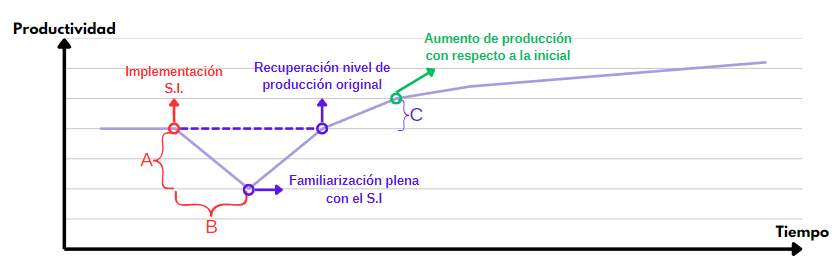
\includegraphics[width=1\textwidth]{img/paradoja.png}
        \vspace{-1.5cm}
    \end{figure}
\end{center}
Se busca que el punto \textcolor{red}{\textbf{A}} y el punto \textcolor{red}{\textbf{B}} tengan el menor valor posible y que el punto \textcolor{violet}{\textbf{C}} tenga el mayor valor posible, esto se puede lograr con:\begin{itemize}
    \item Facilitación de participación.
    \item Facilitación de aprendizaje.
    \item Asistencia de usuario.
\end{itemize}
\subsection{Reingeniería de procesos}
\noindent Rediseño radical de procesos para lograr mejoras significativas en medidas críticas y contemporáneas de rendimiento, como costos, calidad, servicio y rapidez.
\begin{itemize}
    \item \textbf{Objetivos:}
    \begin{itemize}
        \item Reducción de costos.
        \item Mejora de la calidad.
        \item Reducción de tiempos.
        \item Mejora de la satisfacción del cliente.
    \end{itemize}
    \item \textbf{Características:}
    \begin{itemize}
        \item Cambio radical.
        \item Enfocado en procesos.
        \item Mejora de la eficiencia.
        \item Mejora de la eficacia.
        \item Mejora de la calidad.
        \item Mejora de la satisfacción del cliente.
        \item Rapidez, obteniendo resultados en corto plazo.
    \end{itemize}
    \item \textbf{Desventajas:}
    \begin{itemize}
        \item Resistencia al cambio.
        \item Es de alto riesgo.
        \item Despidos debido a la toma de este riesgo.
    \end{itemize}
\end{itemize}
\subsection{Industria 4.0}
\noindent Es la cuarta revolución industrial, se caracteriza por la digitalización de la industria. Se basa en la interconexión de sistemas ciber-físicos, la inteligencia artificial, la robótica, el big data, la computación en la nube, la realidad aumentada, la impresión 3D, la ciberseguridad, la internet de las cosas, la simulación y la integración de sistemas.
\begin{itemize}
    \item \textbf{Características:}
    \begin{itemize}
        \item Productor tiene conciencia del cambio en su forma de trabajar y el cliente mejora el producto final.
        \item Aumento en la seguridad de los trabajadores.
        \item Mejora toma decisiones (Bases digitales).
        \item Aumento de competitividad.
    \end{itemize}
    \item \textbf{Riesgos:}
    \begin{itemize}
        \item Dependencia tecnológica (Brecha digital).
        \item Posibilidad de ataques cibernéticos.
        \item Aumento despidos y contrataciones selectivas.
        \item Resistencia al cambio.
    \end{itemize}
\end{itemize}

\subsection{Transformación digital}
\noindent Implementación de las tecnologías digitales en las empresas para cambiar la forma en que se hacen las cosas. \\
\begin{minipage}{0.45\textwidth}
    \begin{itemize}
        \item \textbf{Características:}
        \begin{itemize}
            \item Mejora la productividad.
            \item Mejora la experiencia del cliente.
            \item Reduce los costos operativos.
        \end{itemize}
    \end{itemize}
\end{minipage}
\hspace{1cm}
\begin{minipage}{0.45\textwidth}
    \begin{itemize}
        \item \textbf{Desventajas:}
        \begin{itemize}
            \item Alto nivel de competitividad.
            \item Necesidad de una evolución constante en la industria.
            \item Impacto en el ámbito cultural de las personas.
        \end{itemize}
    \end{itemize}
\end{minipage}


\subsection{Internet de las cosas (IOT)}
\noindent El IOT es una herramienta que permite la interconexión de objetos cotidianos a la red, permitiendo la comunicación entre ellos y la recolección de datos. Esta herramienta se aplica a la vida cotidiana y a la industria.

\begin{itemize}
    \item \textbf{Características:}
    \begin{itemize}
        \item Conectividad con la red.
        \item Sensibilidad en parámetros analizables.
        \item Interacción entre elementos a través de interfaces para el usuario.
        \item Nivel de seguridad.
        \item Automatización de tareas y optimización de procesos industriales.
    \end{itemize}
    \item \textbf{Ventajas:}
    \begin{itemize}
        \item Mejora la eficiencia.
        \item Mejora la calidad de vida.
        \item Mayor facilidad en el seguimiento de procesos para las empresas.
        \item Optimización de tiempos.
    \end{itemize}
    \item \textbf{Desventajas:}
    \begin{itemize}
        \item Vulnerabilidad en la seguridad.
        \item Costos de implementación.
        \item Dependencia de la tecnología (Brecha digital).
        \item Resistencia cultural por parte del usuario.
    \end{itemize}
\end{itemize}

\newpage


\section{\textcolor{green}{Proceso de desarrollo de S.I (CFOEAR)}}

\subsection{Conceptos}
\noindent Todos los sistemas en su procesos de desarrollo pasan por estos 4 puntos:
\begin{enumerate}
    \item \textbf{Concepción:} Alguien pide o desarrolla la idea de un sistema.
    \item \textbf{Diseño:} Se diseña el sistema tomando en cuenta todos los aspectos y variables.
    \item \textbf{Construcción:} Se construye el sistema siguiendo el diseño.
    \item \textbf{Implementación:} Se implementa en el entorno para el que se creo.
\end{enumerate}
\subsection{Fuentes de solicitudes de proyectos de sistemas de información}
    \begin{itemize}
        \item \textbf{Internas:}
        \begin{itemize}
            \item Jefes de departamento.
            \item Altos ejecutivos.
            \item Especialistas
            \item Usuarios
        \end{itemize}
        \item \textbf{Externas} 
    \end{itemize}
\subsection{Orígenes de proyectos de sistemas de información}
% \vspace{1cm}
\begin{itemize}
    \item \textbf{Integración.} Integrar sistemas nuevos en sistemas aislados de la empresa; \underline{Tecnico}.
    \item \textbf{Velocidad de procesamiento.} Aumentar la velocidad de procesamiento de la información; \underline{Tecnico}.
    \item \textbf{Seguridad/Confidencialidad.} Información accesible y confidencial para algunas personas; \underline{Tecnico}.
    \item \textbf{Exactitud y consistencia.} Para sistemas de información que manejan datos numéricos el sistema debe ser exacto y consistente; \underline{Tecnico}.
    \item \textbf{Confiabilidad.} Manejo y almacenamiento de información en caso de imprevistos; \underline{Tecnico}.
    \item \textbf{Imagen.} Imitar competencia; \underline{Subjetivo}
\end{itemize}
\newpage
\subsection{Estrategias de desarrollo de sistemas de información}
\subsubsection{Ciclo de vida tradicional/lineal/Cascada}
\noindent Conjunto de actividades que tienen que completarse para llevar a cabo un sistema de información. \linebreak
\textbf{Actividades:}
\begin{center}
    \begin{tikzpicture}
        \node[font=\bfseries] (A) at (0,0)  {\hyperlink{def_probl}{Definición del problema}};
        \node[font=\bfseries] (B) at (0,-1) {\hyperlink{est_fac}{Estudio de factibilidad}};
        \node[font=\bfseries] (C) at (0,-2) {\hyperlink{ana_sis}{Análisis del sistema}};
        \node[font=\bfseries] (D) at (0,-3) {\hyperlink{dis_log}{Diseño lógico}};
        \node[font=\bfseries] (E) at (0,-4) {\hyperlink{dis_fis}{Diseño físico}};
        \node[font=\bfseries] (F) at (0,-5) {\hyperlink{con}{Construcción}};
        \node[font=\bfseries] (G) at (0,-6) {\hyperlink{imp}{Implementación}};
        \node[font=\bfseries] (H) at (0,-7) {\hyperlink{rev_pos}{Revisión post-implementación}};
        \node[font=\bfseries] (I) at (0,-8) {\hyperlink{man}{Mantenimiento}};

        \draw[->] (A) -- (B);
        \draw[->] (B) -- (C);
        \draw[->] (C) -- (D);
        \draw[->] (D) -- (E);
        \draw[->] (E) -- (F);
        \draw[->] (F) -- (G);
        \draw[->] (G) -- (H);
        \draw[->] (H) -- (I);
    \end{tikzpicture}
\end{center}

\begin{enumerate}
    \item \hypertarget{def_probl}{\textbf{Definición del problema:}} Se define el problema a resolver.
        \begin{itemize}
            \item Estudio de la situación actual.
            \item Identificación del problema.
            \item Objetivos del sistema (Han de resolver la problemática; Generalmente están acompañados por un verbo).
            \item Limites del sistema (Se definen para evitar que el proyecto se salga de control).
            \item Ámbito del sistema (A que zona de la pirámide apoya).
            \item Bases del sistema (Aspectos legales; No todos los problemas tienen).
            \item Requerimientos del sistema (Que se espera del sistema).
                \begin{itemize}
                    \item Requerimientos de información (Que información maneja el sistema).
                    \item Requerimientos técnicos (Hardware, software y recursos humanos).
                    \item Requerimientos funcionales (Estadísticas, gráficas y cosas que el sistema puede crear con los datos que maneja).
                    \item Requerimientos de seguridad (Claves y niveles de acceso).
                \end{itemize}
        \end{itemize}
    \item \hypertarget{est_fac}{\textbf{Estudio de factibilidad:}} Se estudia si es factible realizar el proyecto.
        \begin{itemize}
            \item Estudio de factibilidad operativo. (Estudio de las areas que afectaría el SI e interesados en el mismo)
            \item Estudio de factibilidad técnico. (Si se tiene la capacidad de obtener HW, SW y/o RRHH necesarios)
            \item Estudio de factibilidad económico (Calculo y establecimiento de costos y beneficios donde: $Costos < Beneficios$).
        \end{itemize}
    \item \hypertarget{ana_sis}{\textbf{Análisis del sistema:}} Una vez se confirma la factibilidad del proyecto se proceden a analizar las entradas, procesos y salidas que conformaran el sistema para su funcionamiento.
    \item \hypertarget{dis_log}{\textbf{Diseño lógico:}} Se diseña el sistema en base a los requerimientos del sistema. Este diseño puede ser de 4 tipos:
        \begin{itemize}
            \item Diagrama de flujo de datos (DFD): Sirven para modelar procesos y muestra como se mueve la información.
            \item Diseño de procedimientos administrativos: Elementos necesarios para llevar a cabo una función administrativa resumido en un documento.
            \item Diseño de sistemas de codificación: Representación en caracteres de la información para evitar el uso de largas cadenas de codificación. Existen varios tipos de codificación:
            \begin{itemize}
                \item Secuencial: Cada elemento tiene un número y se ordenan de menor a mayor. Fácil de codificar pero dificulta la búsqueda de datos.
                \item Por bloque: Se agrupan los elementos en bloques y se les asigna un número. Facilita la búsqueda de datos como en un indice.
                \item De consonantes: Se basa en la eliminación de las consonantes después de la primera consonante de cada palabra.
                \begin{tcolorbox}[colback=green!10!white,colframe=green!75!black,title=Ejemplo de codificación de consonantes]
                    \begin{center}
                        \begin{tabular}{|c|c|}
                            \hline
                            \textbf{Nombre} & \textbf{Codificación} \\ \hline
                            Ingeniería & Ingnr \\ \hline
                            Informática & Infrm \\ \hline
                            Computación & Cmptc \\ \hline
                        \end{tabular}
                    \end{center}
                \end{tcolorbox}
                \item Nemotécnico: Uno de los tipos de codificación mas usados, se basa en la creación de una palabra clave para cada elemento.
                Sin embargo dependiendo de la codificación esta palabra clave puede significar mas de una cosa, lo que nunca puede pasar.
                \begin{tcolorbox}[colback=green!10!white,colframe=green!75!black,title=Ejemplo de codificación Nemotécnica]
                    \begin{center}
                        \begin{tabular}{|c|c|}
                            \hline
                            \textbf{Nombre} & \textbf{Codificación} \\ \hline
                            Universidad del Bio Bio & UBB \\ \hline
                            Universidad de Concepción & UDEC \\ \hline
                            Universidad de Santiago & USACH \\ \hline
                        \end{tabular}
                    \end{center}
                \end{tcolorbox}
                \item Por grupos: Se agrupan elementos en grupos que poe si solos tienen un significado, pero el conjunto de estos grupos también tiene un significado. Facilita la búsqueda de datos al igual que un indice.
                \begin{tcolorbox}[colback=green!10!white,colframe=green!75!black,title=Ejemplo de codificación Por grupos]
                    \begin{center}
                        \begin{tabular}{|c|c|}
                            \hline
                            \textbf{Nombre} & \textbf{Codificación} \\ \hline
                            Ingeniería & T \\ \hline
                            Civil & 1 \\ \hline
                            En Ejecución & 2 \\ \hline
                            Informática & I0 \\ \hline
                            Biomédica & B0 \\ \hline
                        \end{tabular}
                        \\[0.5cm]
                        T1I0 $\rightarrow$ Ingeniería Civil Informática \\
                        T1B0 $\rightarrow$ Ingeniería Civil Biomédica \\
                        T2I0 $\rightarrow$ Ingeniería En Ejecución Informática
                    \end{center}
                \end{tcolorbox}
            \end{itemize}
            \item Diseño conceptual E/S (Entrada/Salida): Se diseña la forma en que se ingresaran los datos al sistema y como se mostraran los resultados.
            \begin{figure}[H]
                \centering
                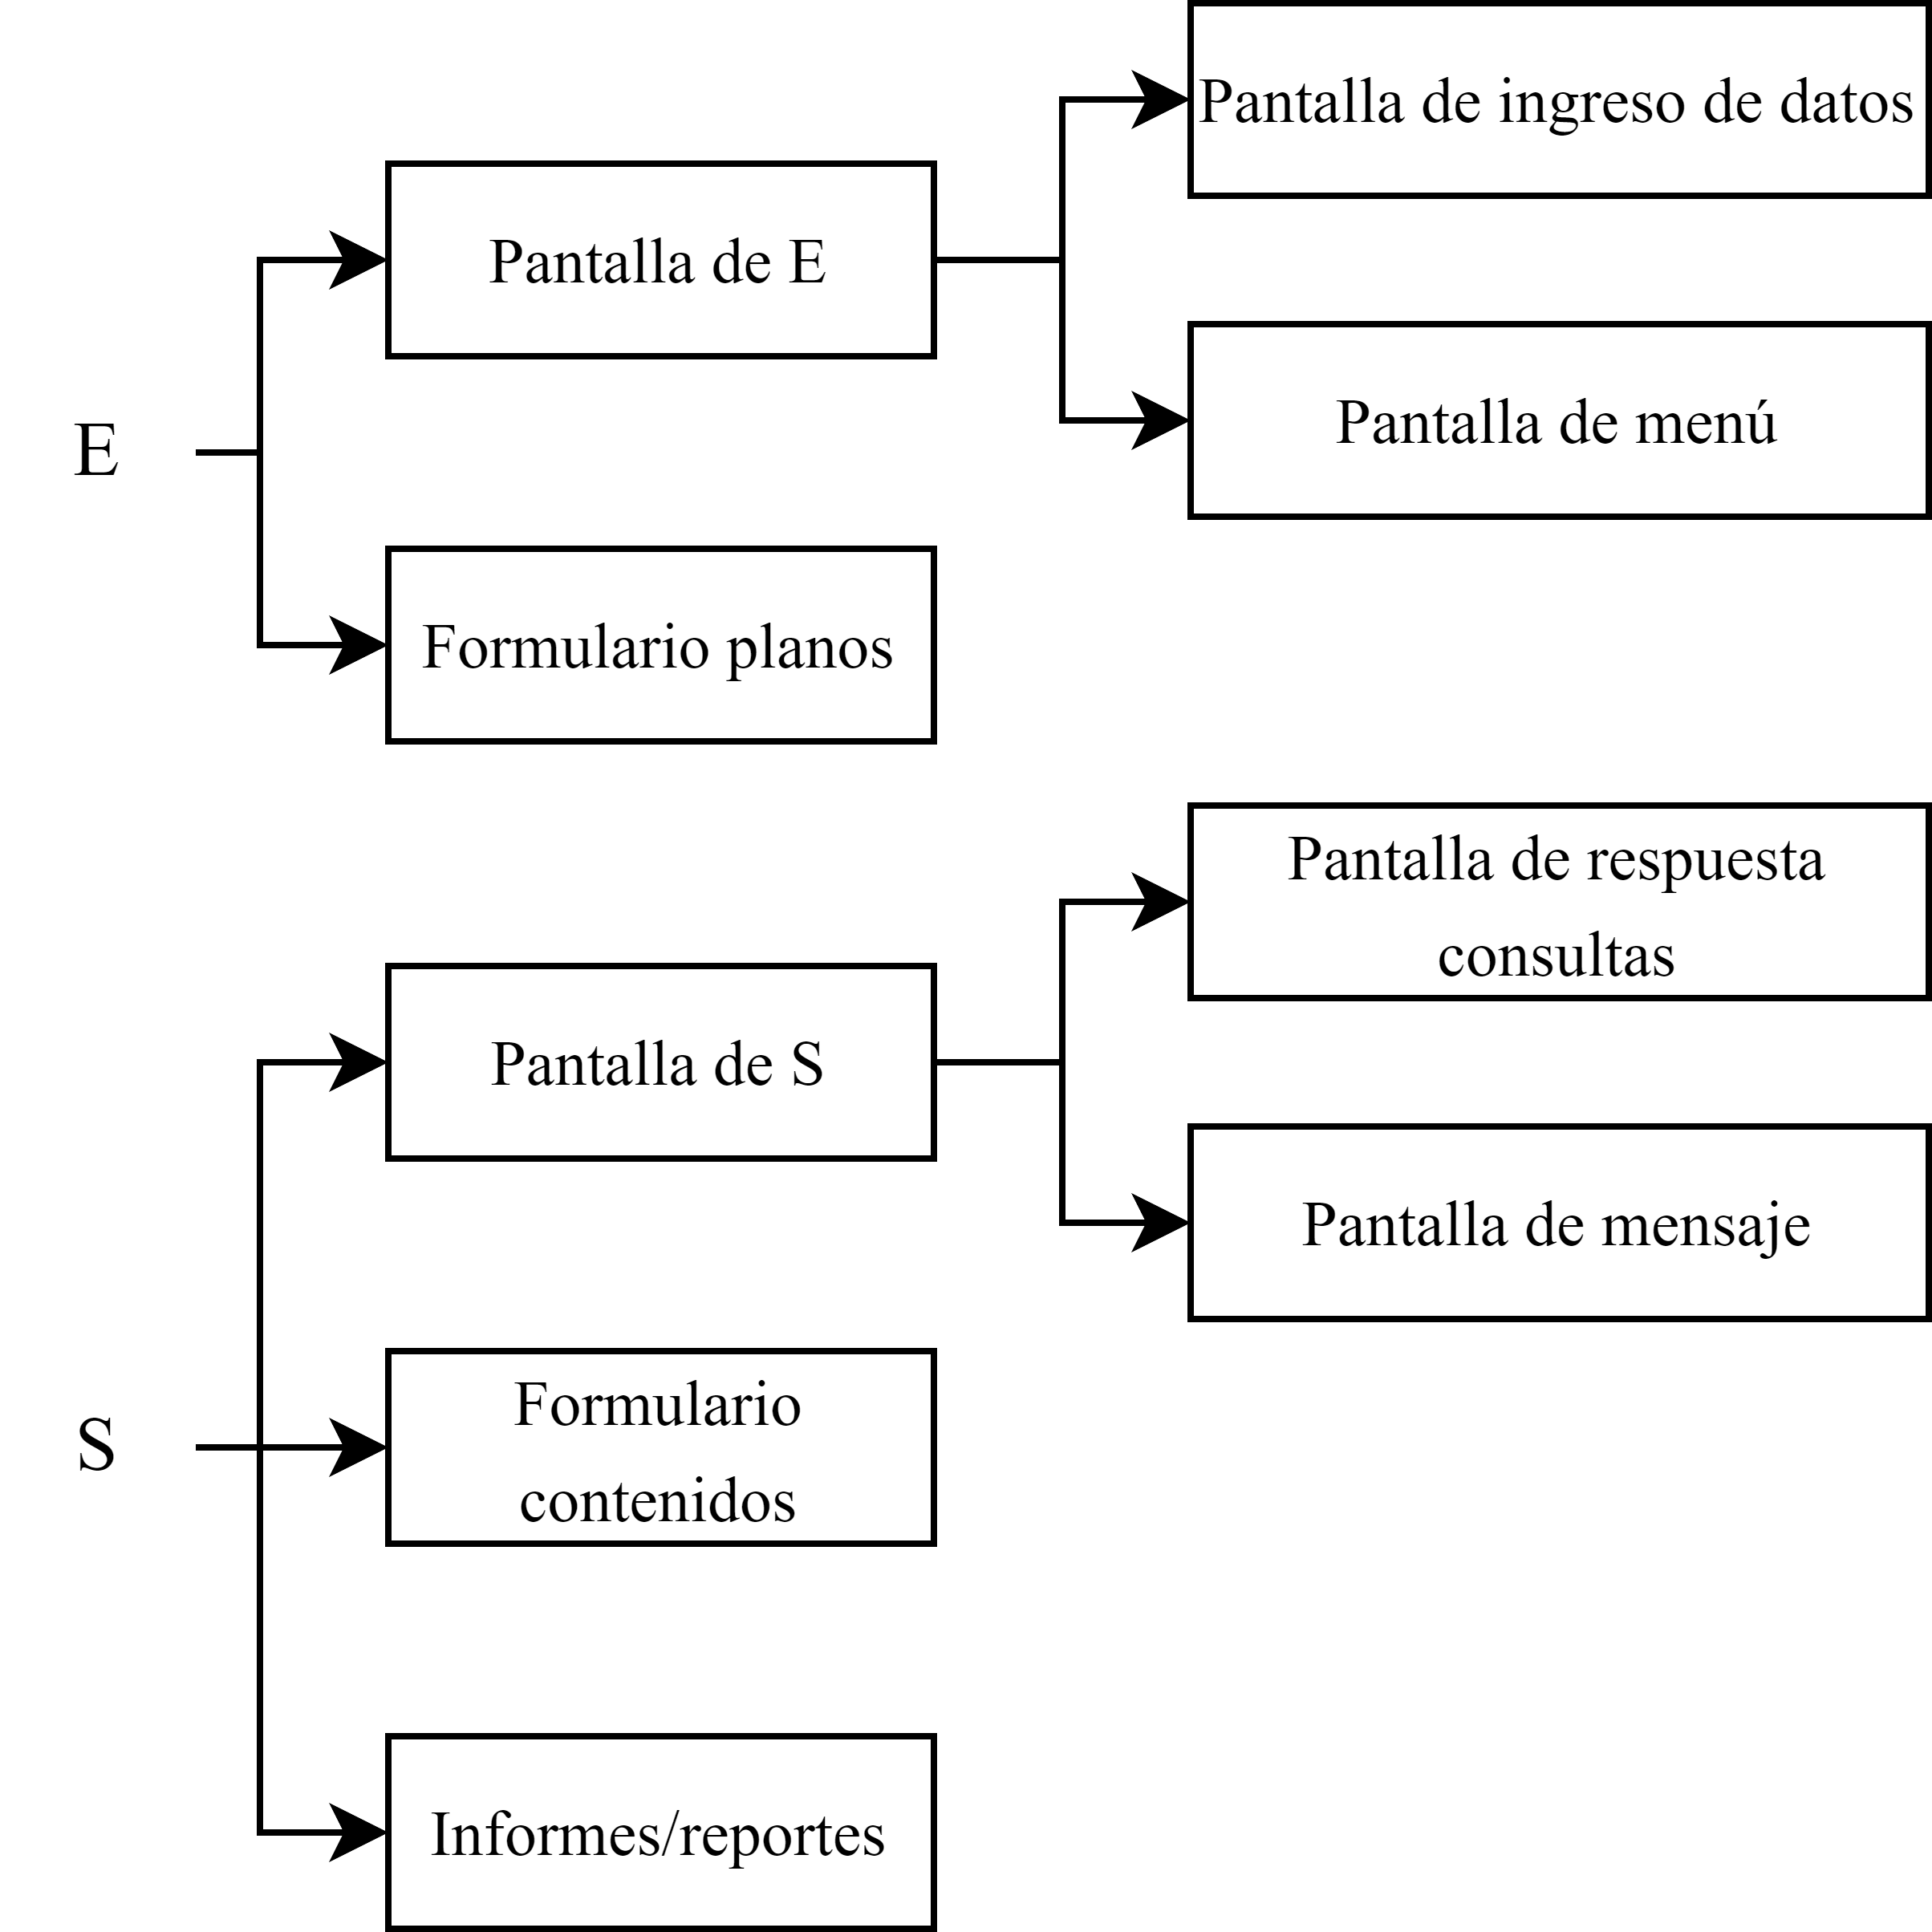
\includegraphics[width=0.5\textwidth]{img/DConceptual.png}
            \end{figure}
        \end{itemize}
    \item \hypertarget{dis_fis}{\textbf{Diseño físico:}} Se diseña el sistema en base a la información que se tiene como objetivo manejar.
    \begin{itemize}
        \item Diseño físico E/S. (Exacto lo que se ve en el computador)
        \item Diseño de base de datos (MER/Modelo de datos).
        \item Diseño jerarquía de menus (Que acción esta por sobre otra y cual lleva a otra).
    \end{itemize}
    \item \hypertarget{con}{\textbf{Construcción:}} Punto en el cual se procede en la selección del lenguaje sobre el cual trabajaremos, el que utilizaremos para crear un programa y someterlo a pruebas de funcionamiento. 
        El objetivo de probar el programa es lograr un programa fiable y que cumpla con los requerimientos del sistema (que no se caiga) y asi poder entregar un sistema completamente funcional. \\\\
    \item \hypertarget{imp}{\textbf{Implementación:}}
        \begin{itemize}
            \item Poblado de base de datos: Ingreso de datos necesarios para el funcionamiento del sistema, siendo estos datos requerimientos de información.
            \item Entrenamiento/capacitación de usuarios: Enseñar al usuario a usar los datos del sistema.
            \begin{itemize}
                \item Usuarios a capacitar.
                \item Responsable capacitación.
                \item Recursos necesarios.
                \item Plan de capacitación. 
            \end{itemize}
            \item Puesta en marcha: Poner en funcionamiento el sistema, existen 4 formas de poner en marcha un sistema:            
            \begin{itemize}
                \item Inmediata: Apenas finaliza el sistema anterior, el nuevo sistema entra en funcionamiento (Opción mas arriesgada al momento de poner a prueba el nuevo sistema).
                \begin{figure}[H]
                    \centering
                    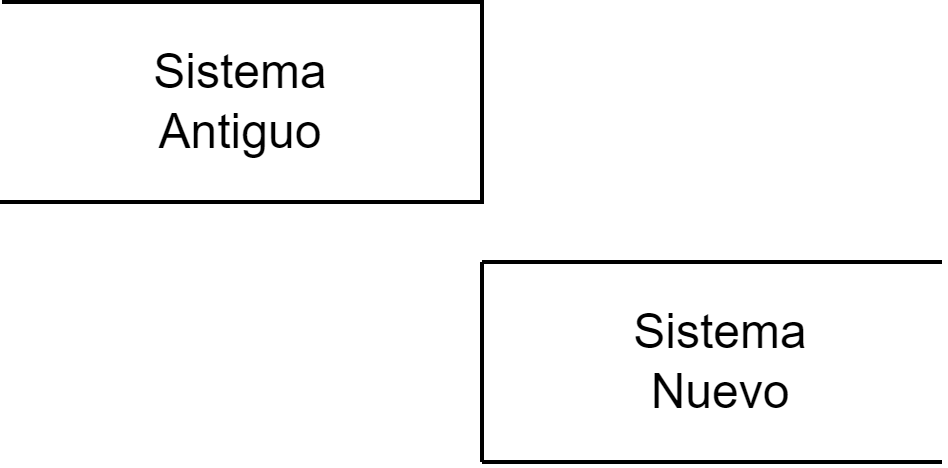
\includegraphics[width=0.4\textwidth]{img/Inmediato.png}
                \end{figure}
                \item Paralela: Mientras el sistema antiguo sigue en funcionamiento, el nuevo sistema se va implementando por completo (Opción mas segura pero consume muchos recursos).
                \begin{figure}[H]
                    \centering
                    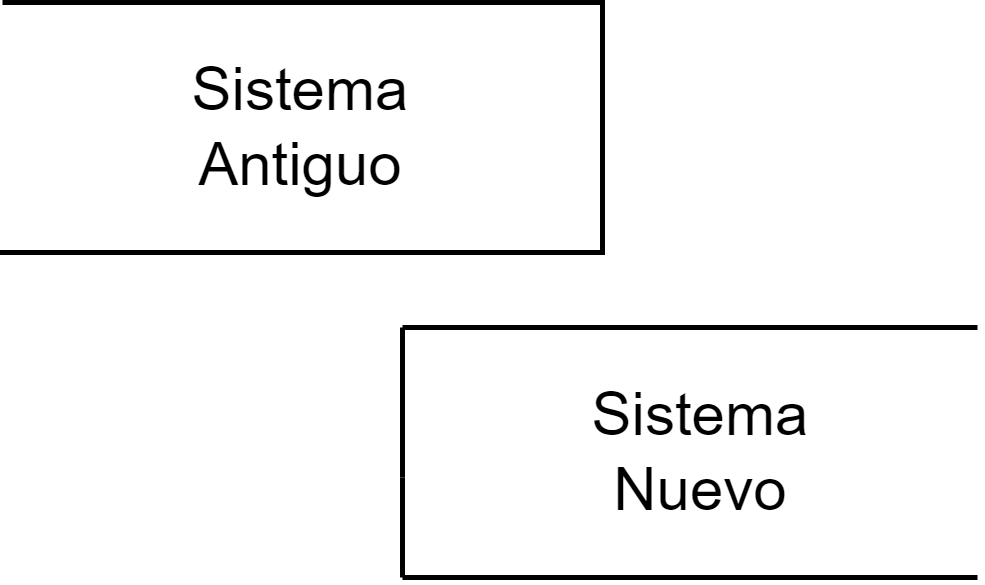
\includegraphics[width=0.4\textwidth]{img/Paralelo.png}
                \end{figure}
                \item Piloto: Se implementa el sistema en una parte de la empresa para ver como funciona (Opción intermedia).
                \begin{figure}[H]
                    \centering
                    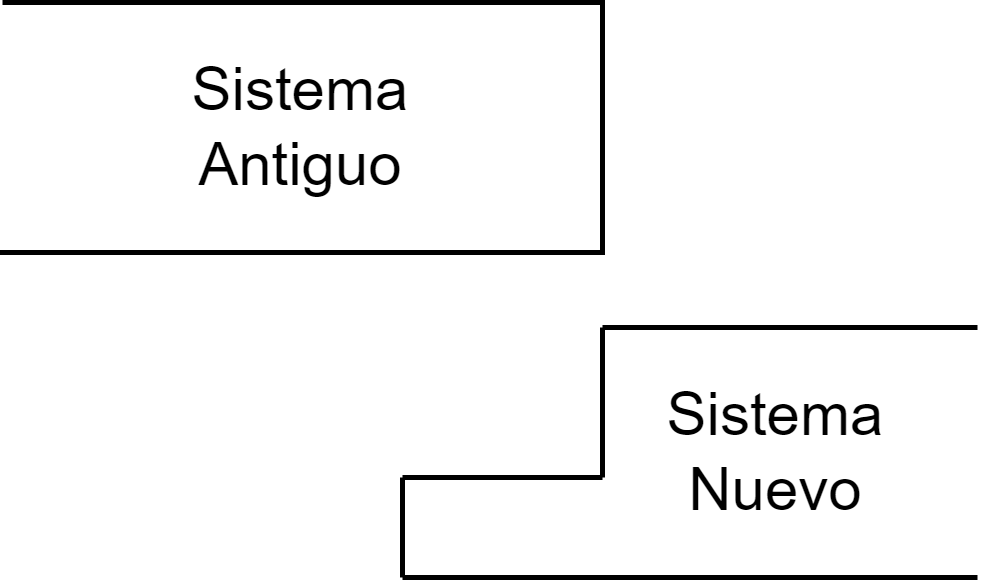
\includegraphics[width=0.4\textwidth]{img/Piloto.png}
                \end{figure}
                \item Gradual: Se implementa el sistema por partes mientras el antiguo sigue en funcionamiento (Opción segura pero no al nivel de la paralela).
                \begin{figure}[H]
                    \centering
                    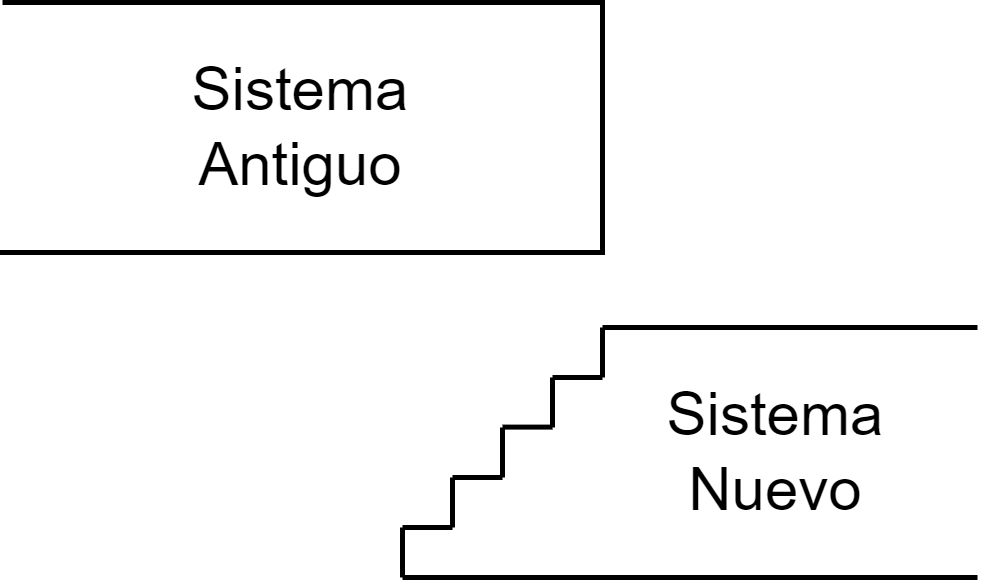
\includegraphics[width=0.4\textwidth]{img/Gradual.png}
                \end{figure}
            \end{itemize}
        \end{itemize}
    \item \hypertarget{rev_pos}{\textbf{Revisión post-implementación:}} Revision del funcionamiento correcto del sistema instalado.
    \item \hypertarget{man}{\textbf{Mantenimiento:}} Proceso de corrección de errores y mejoras del sistema. Existen 4 tipos de mantenimiento:
    \begin{itemize}
        \item Preventiva: Se realiza antes de que ocurra un error.
        \item Correctiva: Se realiza después de que ocurra un error.
        \item Perfectiva: Se realiza para mejorar el sistema.
        \item Adaptativa: Se realiza para adaptar el sistema a cambios en el entorno y sus nuevas tecnologías.
    \end{itemize}
\end{enumerate} 
% \newpage
\subsubsection{Prototipos}
\noindent Alternativa al ciclo de vida tradicional, se basa en la creación de un prototipo para que el cliente pueda ver como se verá el sistema final.
\begin{itemize}
    \item \textbf{Ventajas:}
    \begin{itemize}
        \item Se puede ver el sistema antes de que este terminado.
        \item Se pueden hacer cambios antes de que el sistema este terminado.
        \item Se puede ver si el sistema cumple con los requerimientos.
        \item Se determina mas rápidamente la viabilidad del proyecto.
    \end{itemize}
    \item \textbf{Desventajas:}
    \begin{itemize}
        \item Puede ser costoso.
        \item Puede ser lento.
        \item Puede ser difícil de implementar.
        \item El usuario puede no saber que es lo que quiere.
        \item El usuario debe estar presente en todo momento.\\\\\\
    \end{itemize}
\end{itemize}
\noindent En la creación de un prototipo se deben seguir los siguientes pasos:
\begin{enumerate}
    \item \textbf{Definición de requerimientos:} Se definen los requerimientos del sistema.
    \item \textbf{Análisis y diseño del prototipo:} Se diseña el prototipo.
    \item \textbf{Construcción del prototipo:} Se construye el prototipo.
    En este punto del proceso se pueden dar 4 situaciones:
    \begin{itemize}
        \item La construcción del prototipo no es la esperada por lo que se vuelve al diseño del prototipo.
        \item El prototipo no es el esperado pero ya se identificaron las necesidades del usuario.
        \item El proyecto resulta ser mas grande de lo esperado por lo tanto se descarta el proyecto.
        \item El prototipo es el esperado por lo que se pasa a la etapa de construcción tomando el prototipo como base.
    \end{itemize}
\end{enumerate}
\begin{figure}[H]
    \centering
    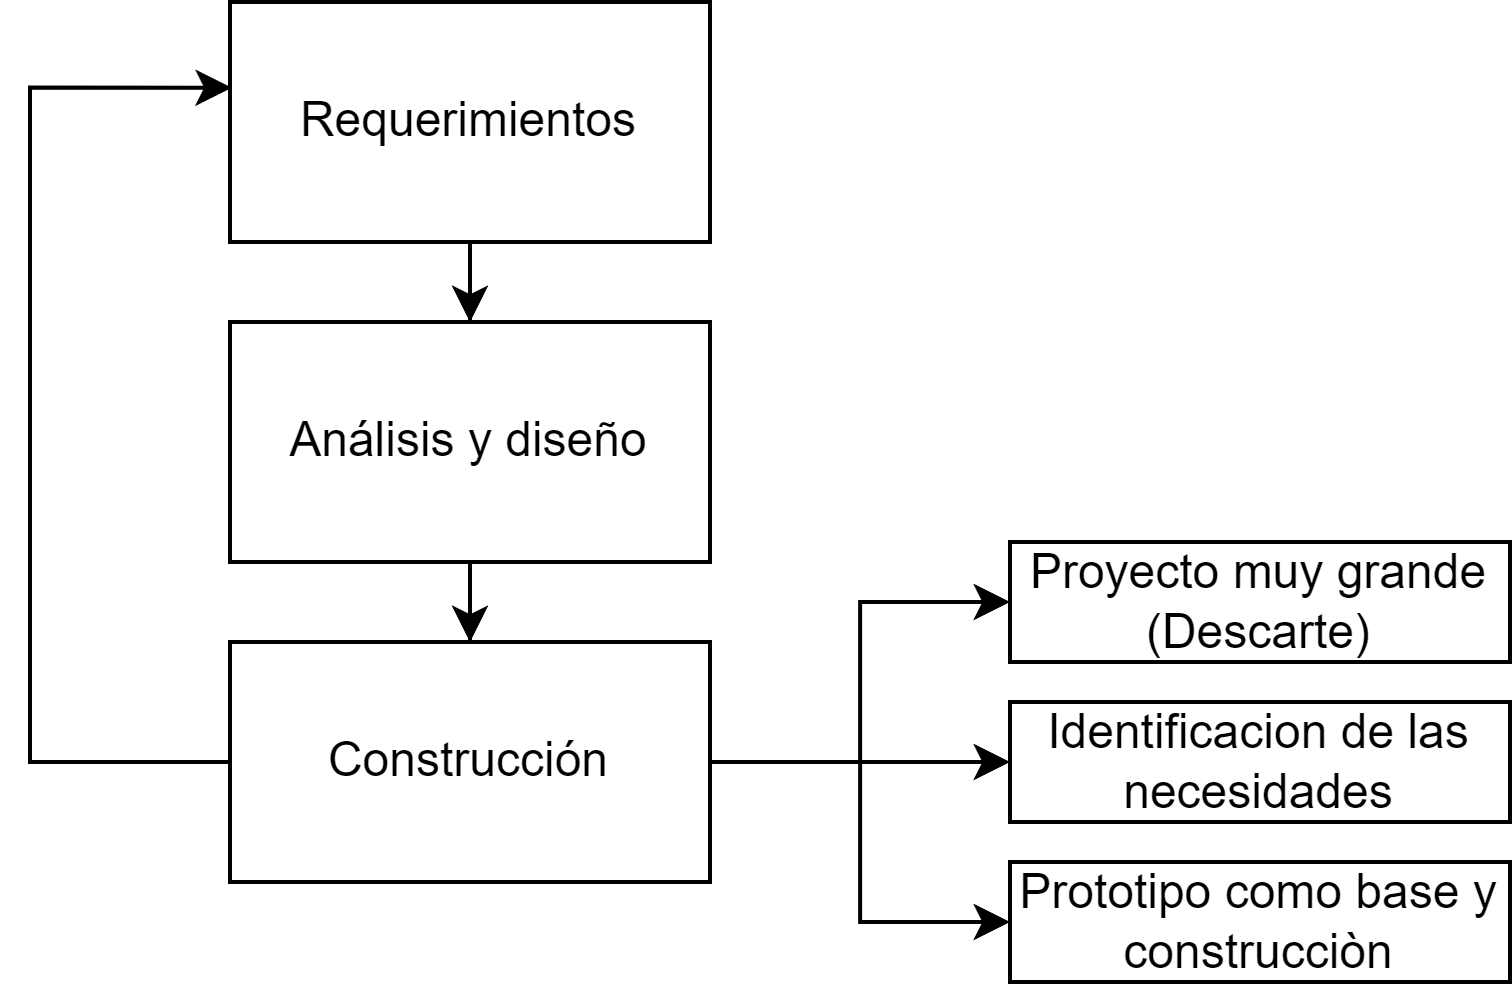
\includegraphics[width=0.45\textwidth]{img/Prototipo.png}
\end{figure}
% \newpage
\subsection{Alternativa de desarrollo del sistema de información}
\noindent Basándose en la identificación de fuentes internas o externas existen otras alternativas para el desarrollo de sistemas de información
\begin{enumerate}
    \item Internas: Fuentes de desarrollo provenientes del mismo entorno empresarial. Pueden ser:
    \begin{itemize}
        \item Agentes internos: Personal perteneciente a la empresa que desarrolla el sistema. Ventajas de recurrir a agentes internos:
        \begin{itemize}
            \item Tienen conocimiento del funcionamiento de la empresa.
            \item La comunicación con estos agentes es mas simple y fluida en comparación con agentes externos. 
        \end{itemize}
    \end{itemize}
    \newpage
    \item Externas: Fuentes de desarrollo provenientes de un entorno empresarial diferente. Pueden ser:
    \begin{itemize}
        \item Agentes externos: Personal no perteneciente a la empresa que desarrolla el sistema. Ventajas de recurrir a agentes externos:
        \begin{itemize}
            \item Tienen experiencia en el desarrollo de sistemas de información.
            \item Pueden aportar nuevas ideas y perspectivas al desarrollo del sistema.
        \end{itemize}
    \end{itemize}
    La opciones que ofrece recurrir a fuentes externas de desarrollo son:
    \begin{itemize}
        \item Comprar un producto existente en el mercado.
        \item Contratar desarrollo.
        \begin{itemize}
            \item Razones:
            \begin{itemize}
                \item Falta de personal calificado.
                \item Para no tener que aumentar el personal de la empresa.
                \item Se pueden concentrar unicamente en el negocio.
                \item Aumenta la velocidad de desarrollo del SI.
            \end{itemize}
            \item Riesgos:
            \begin{itemize}
                \item Perdida de conocimiento y experiencia una vez los agentes externos terminan el sistema.
                \item Dependencia de los agentes externos en caso de fallas en el sistema.
                \item Perdida del control del desarrollo del sistema.
                \item Seguridad de la información y recursos.
                \item Confidencialidad de la información.
                \item Pertenencia del sistema.
            \end{itemize}
            \item Consideraciones:
            \begin{itemize}
                \item Trabajo conjunto entre agentes internos y externos.
                \item Definición de actividades.
                \item Definición de responsabilidades (funcionalidades y atribuciones).
                \item Multa por incumplimiento.
                \item Clausula de pertenencia del sistema.
            \end{itemize}
        \end{itemize}
    \end{itemize}
    \begin{figure}[H]
        \centering
        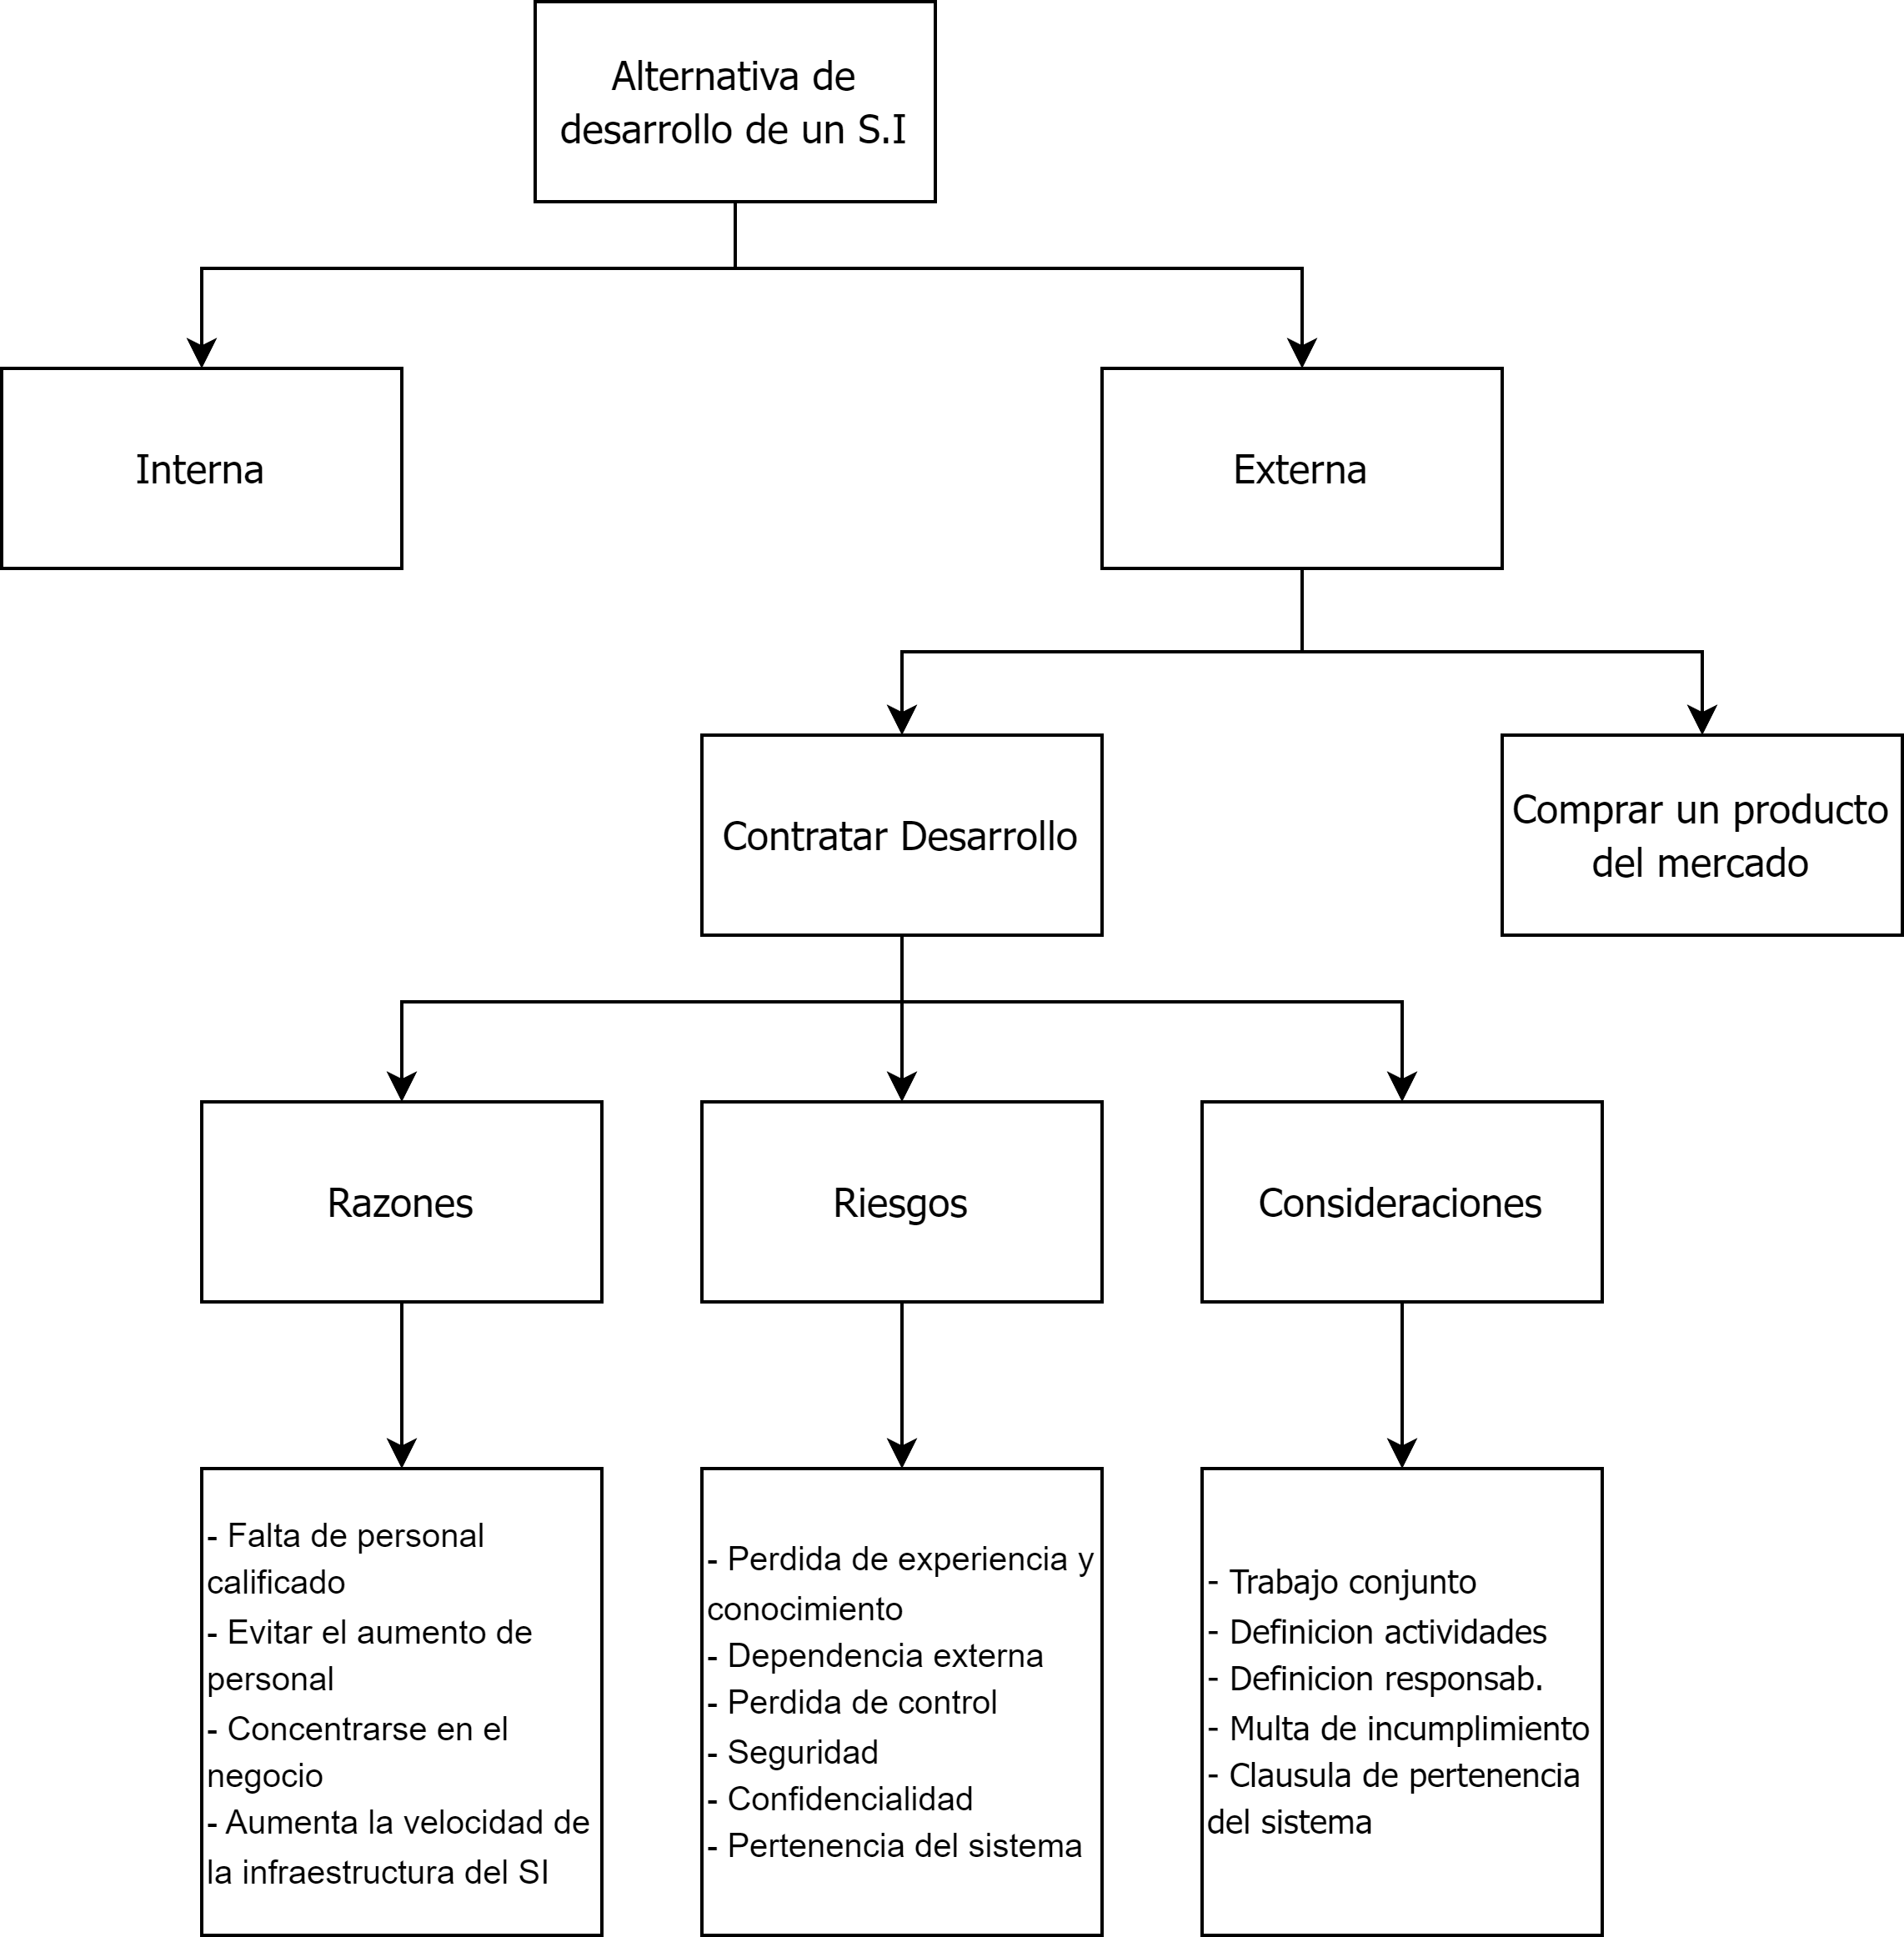
\includegraphics[width=0.72\textwidth]{img/Alt_des_SI.png}
    \end{figure}
\end{enumerate}
\subsection{Restricciones de desarrollo de sistemas de información}
\begin{itemize}
    \item Falta de recursos.
    \begin{itemize}
        \item Humanos
        \item Técnicos (HW, SW)
        \item Económicos
    \end{itemize}
    \item Falta personal calificado.
    \item Falta claridad de necesidad del S.I
    \item Falta de apoyo de dirección.
    \item Falta relevancia para el S.I
    \item Falta cultura informática
\end{itemize}
\newpage
\section{Diagramas de flujo de datos (\textbf{DFD})} 
\noindent Los diagramas de flujo de datos son una herramienta que nos permite modelar procesos y mostrar como se mueve la información. Dentro de los DFD existen 3 niveles:
\begin{itemize}
    \item Diagrama de contexto: Muestra el sistema como una caja negra y las interacciones que tiene con el entorno (No muestra archivos).
    \begin{figure}[H]
        \centering
        \includegraphics[width=0.5\textwidth]{img/contexto.png}
    \end{figure}
    \item Diagrama de nivel superior: Muestra a detalle los procesos y elementos pertenecientes al diagrama de contexto, incluyendo archivos y bases de datos (Muestra archivos).
    \begin{figure}[H]
        \centering
        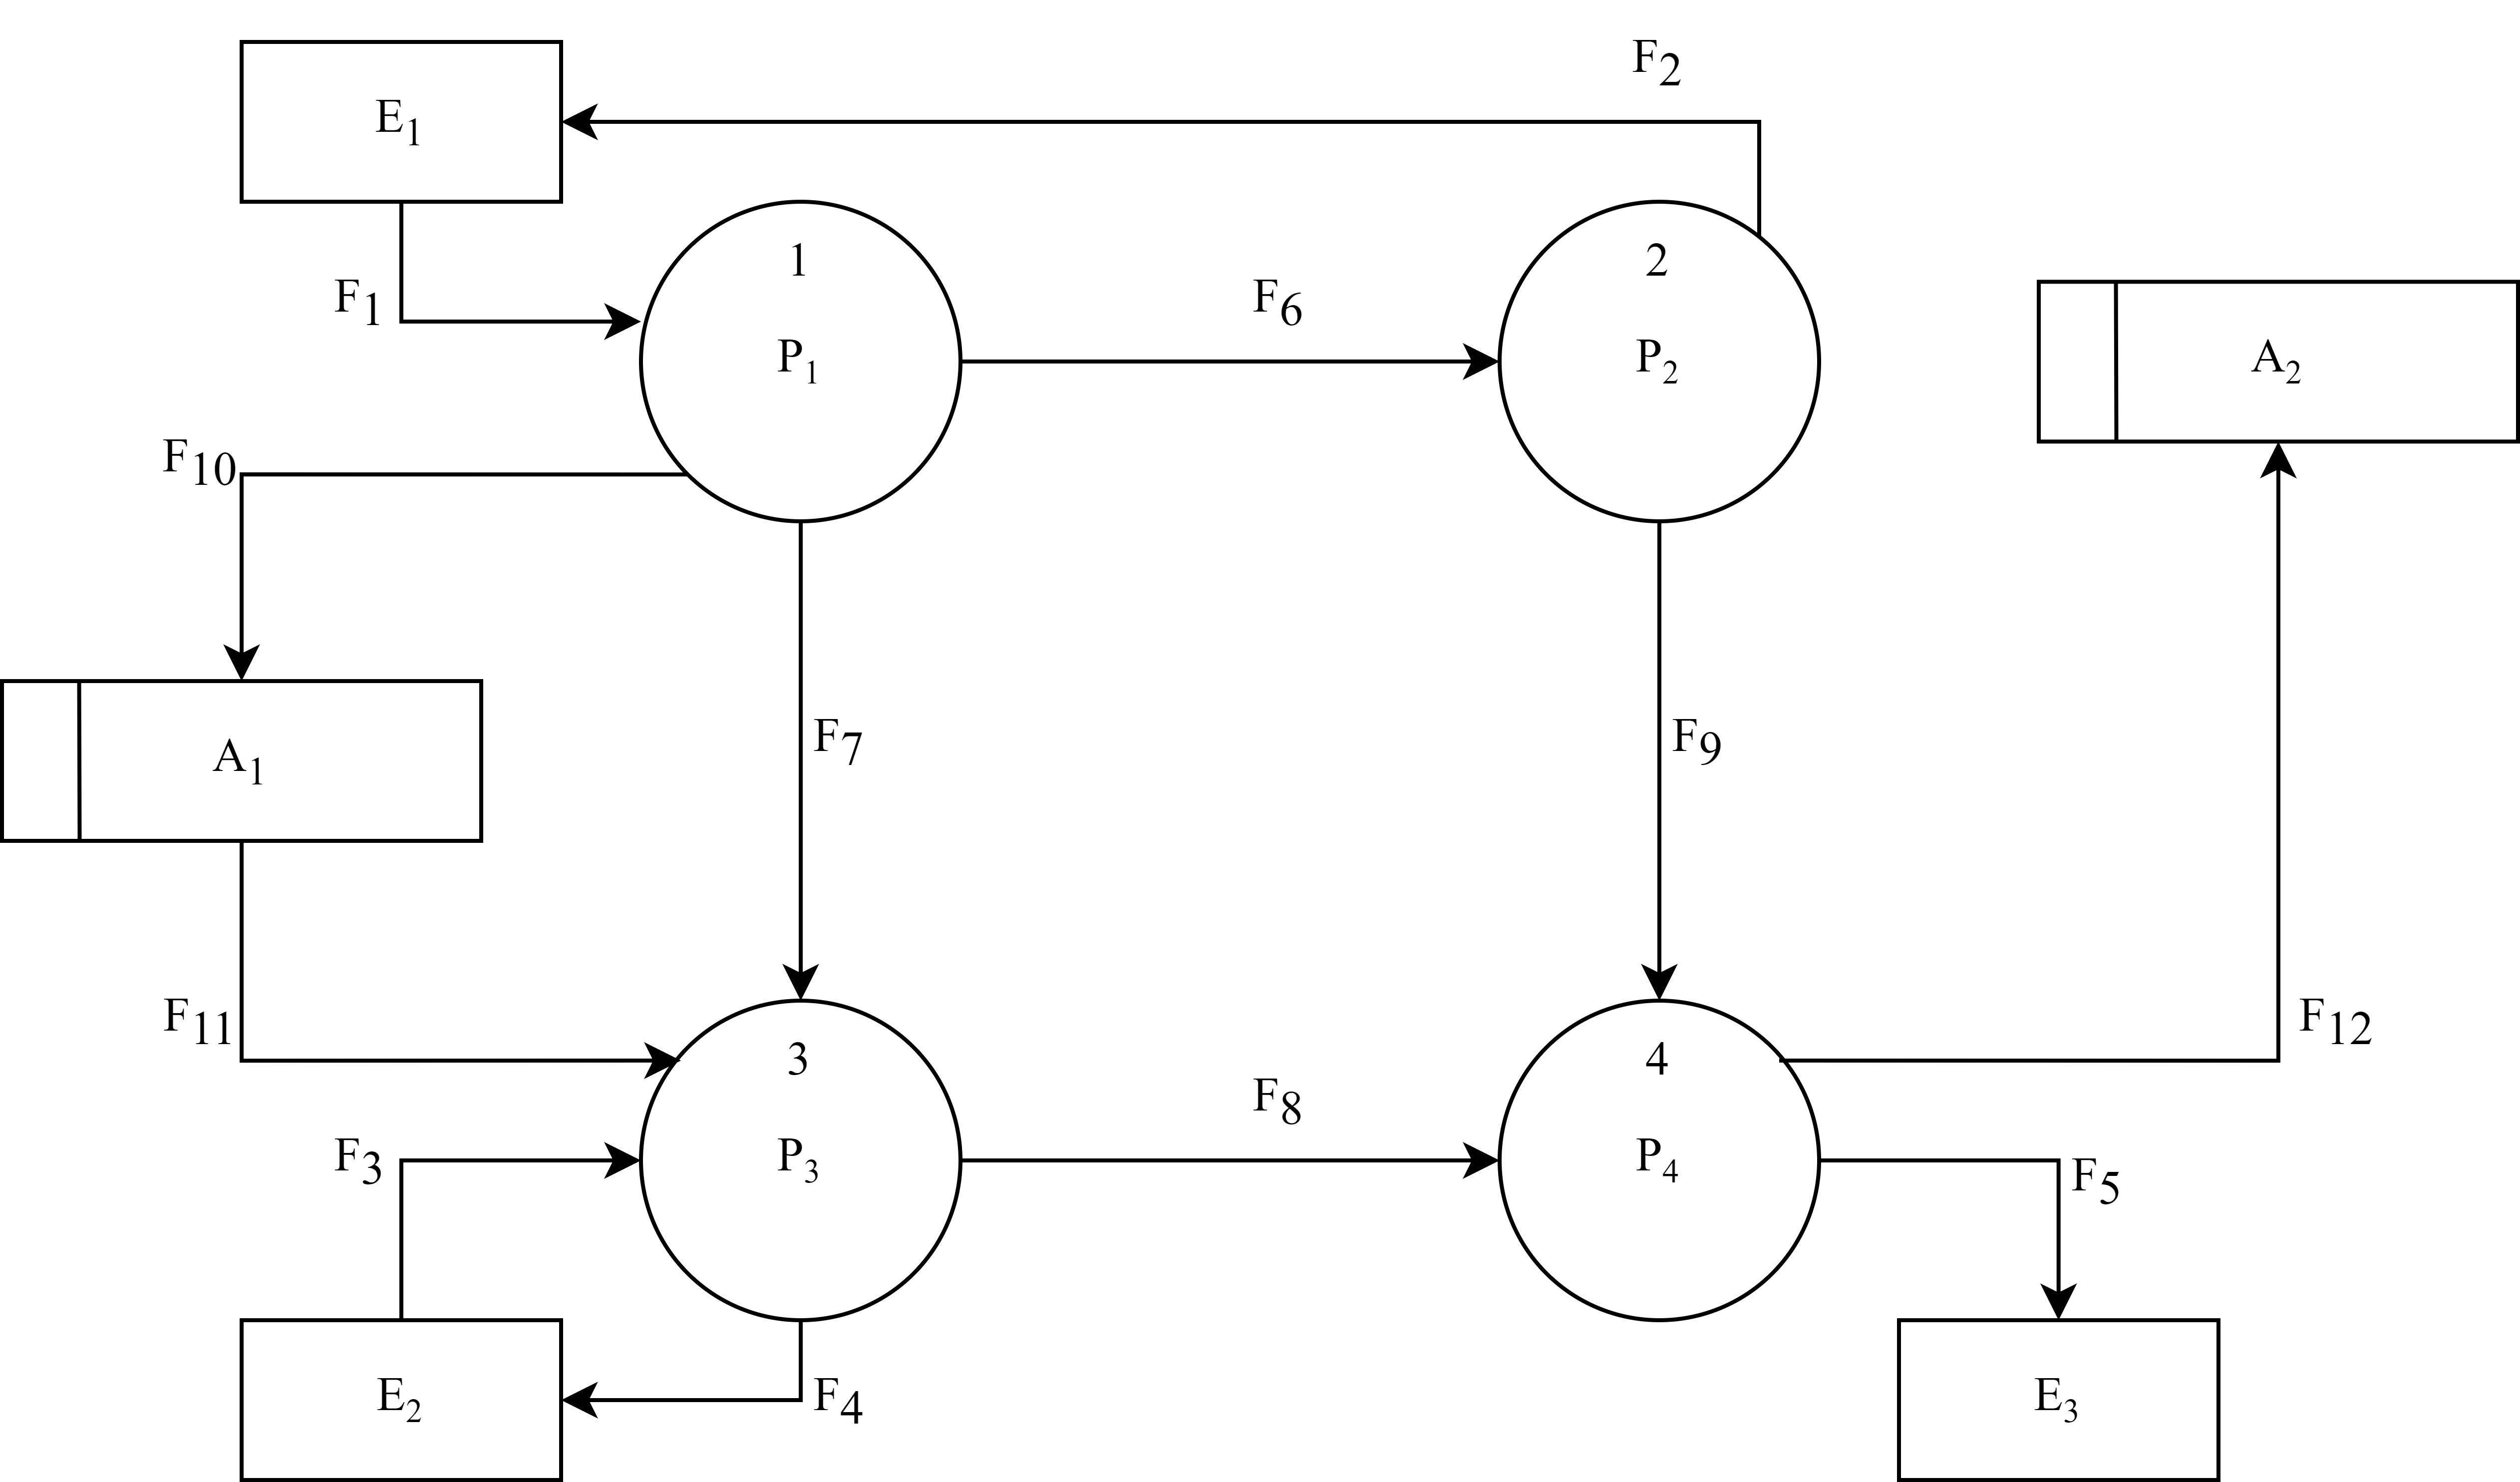
\includegraphics[width=1\textwidth]{img/Superior.png}
    \end{figure}
    \item Diagrama de detalle o expansion: Muestra a detalle los procesos y elementos pertenecientes al diagrama de nivel superior (Conserva archivos y entidades; Procesos superiores se representan de otra forma).
    \begin{figure}[H]
        \centering
        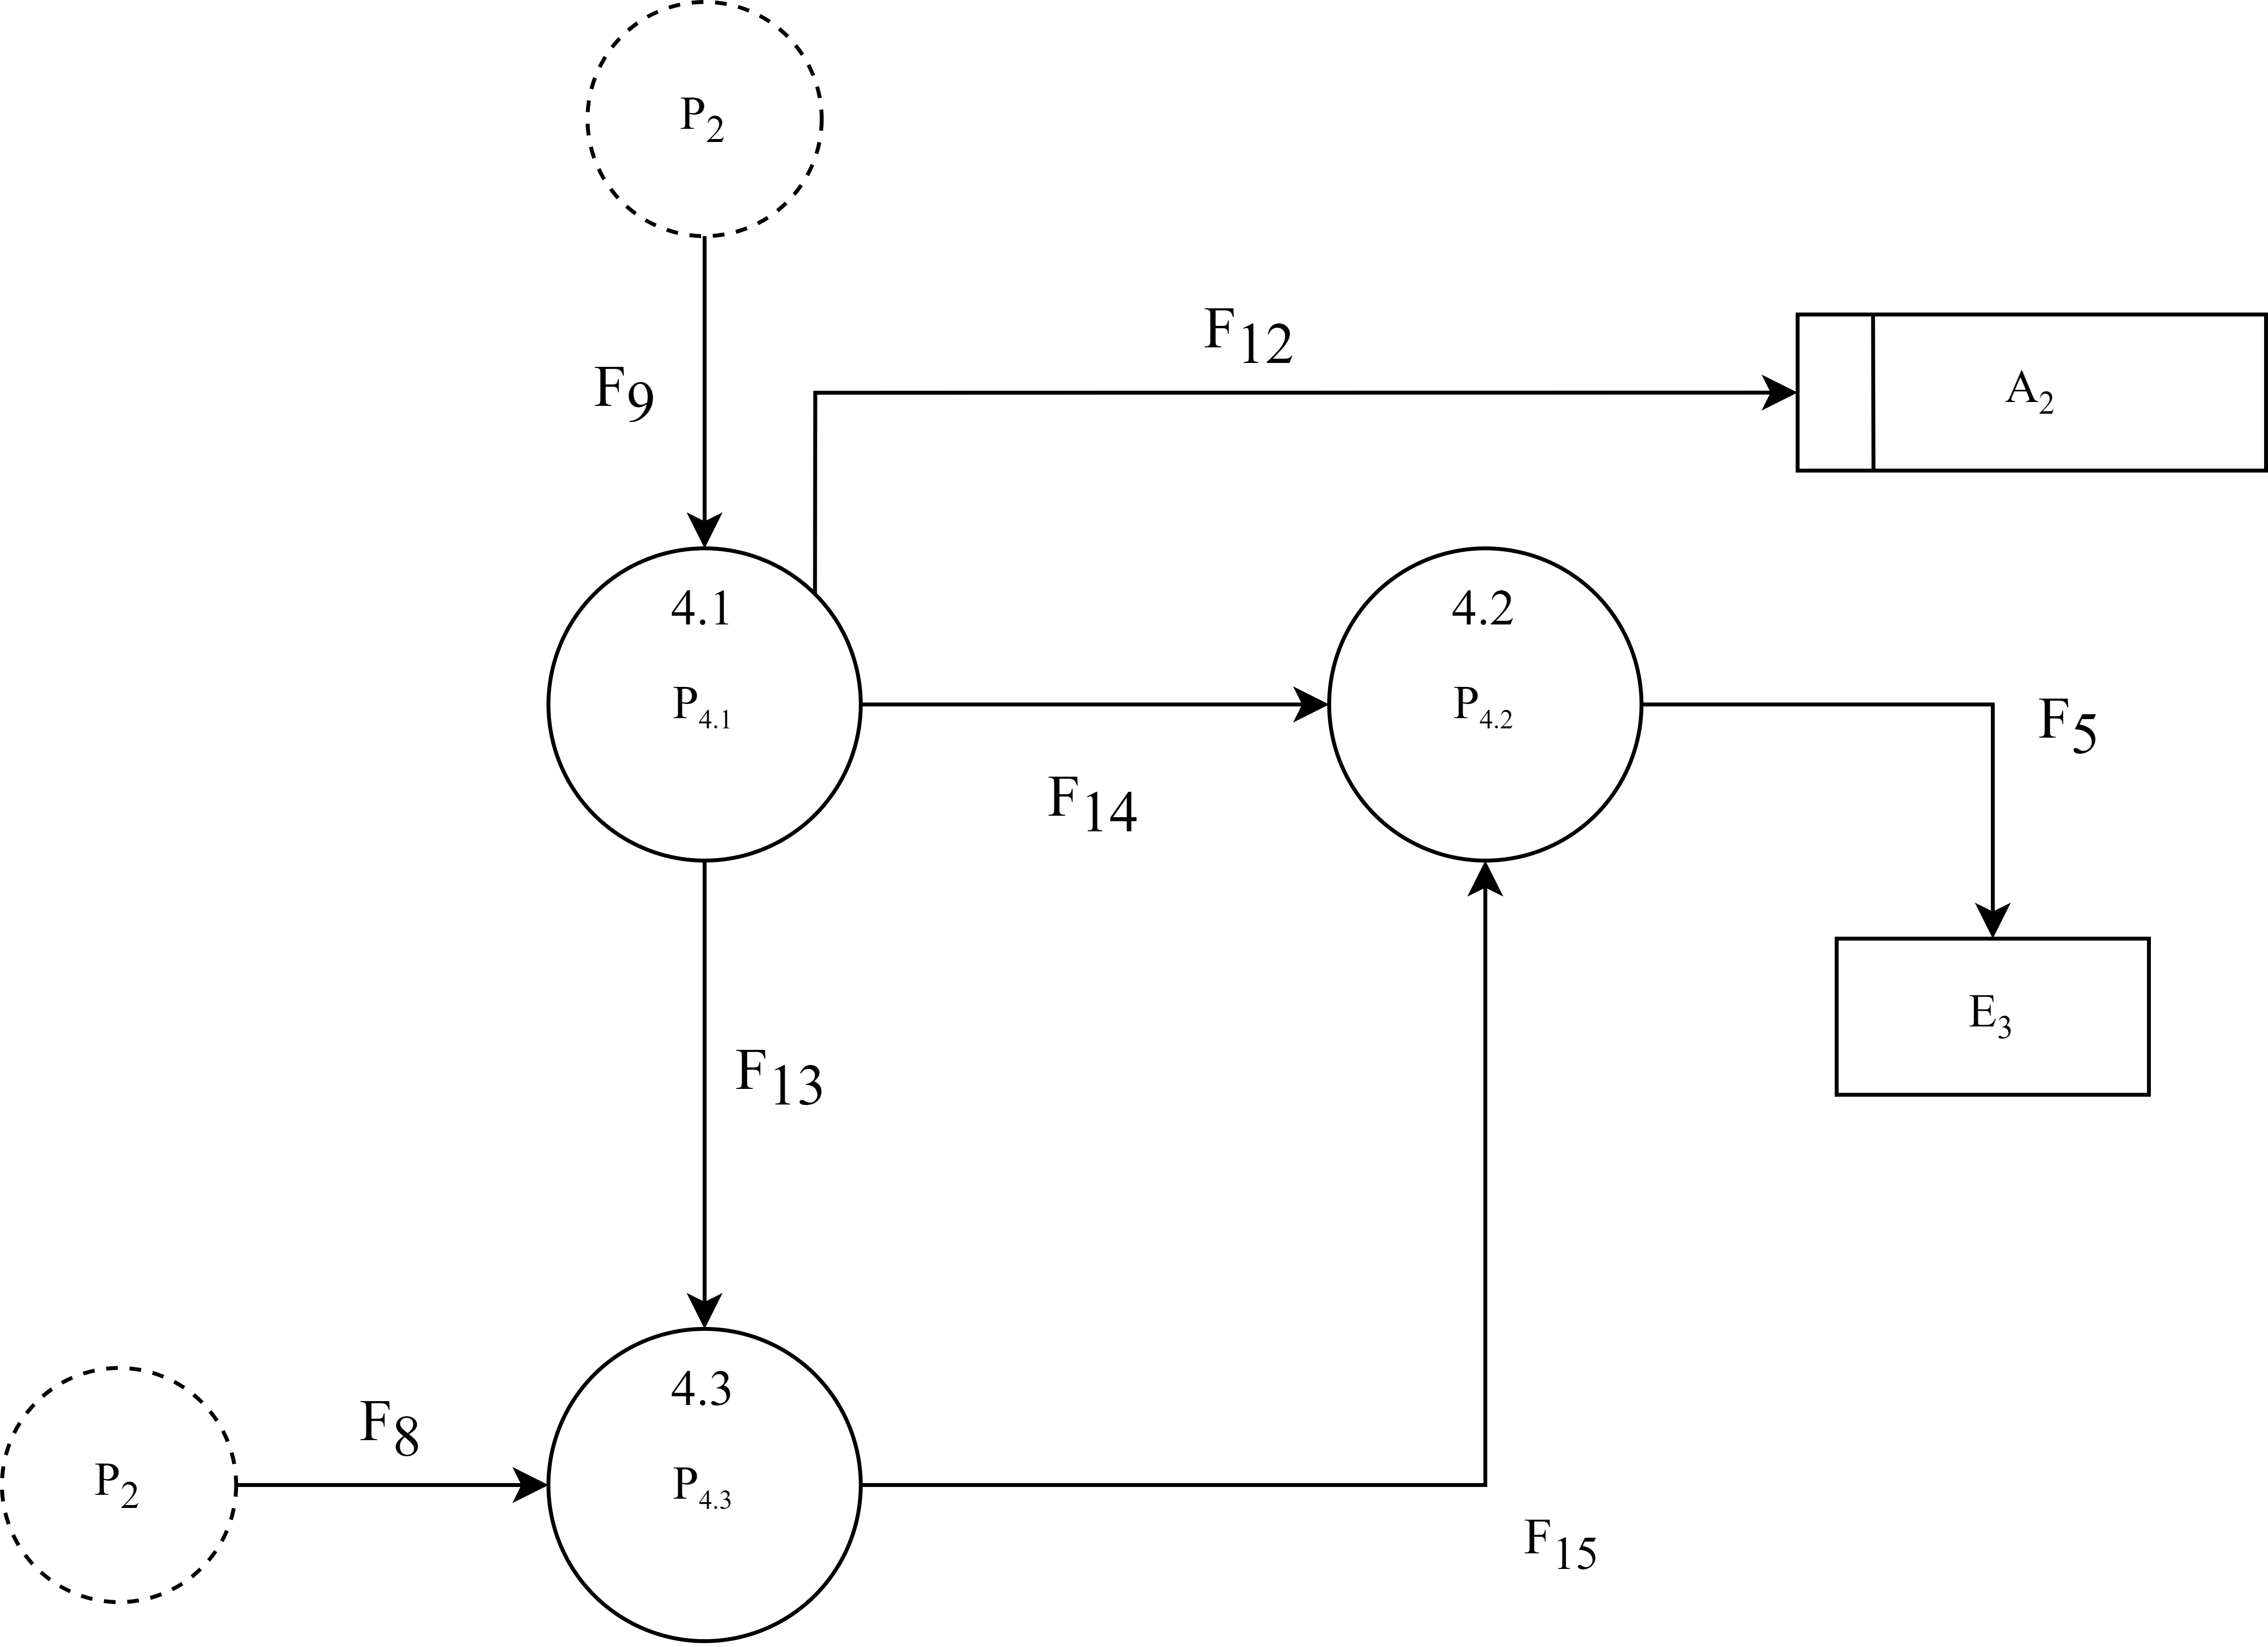
\includegraphics[width=0.7\textwidth]{img/Detallado.png}
    \end{figure}
\end{itemize}
Las figuras que utilizaremos para la construcción de nuestros DFD son:
\begin{figure}[H]
    \centering
    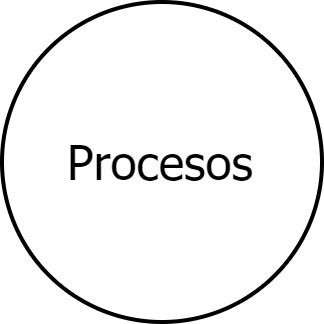
\includegraphics[width=0.20\textwidth]{img/procesos.png}\hspace{1.5cm}
    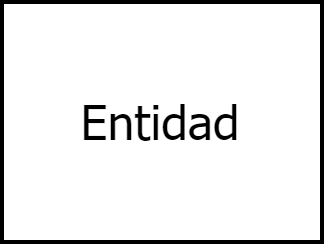
\includegraphics[width=0.23\textwidth]{img/entidad.png}\hspace{1.5cm}
    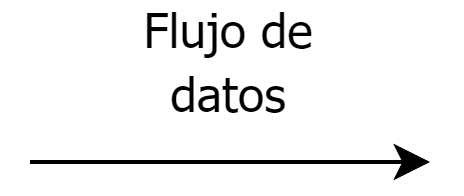
\includegraphics[width=0.30\textwidth]{img/flujo.png}\hspace{1.5cm}
\end{figure}
\begin{figure}[H]
    \centering
    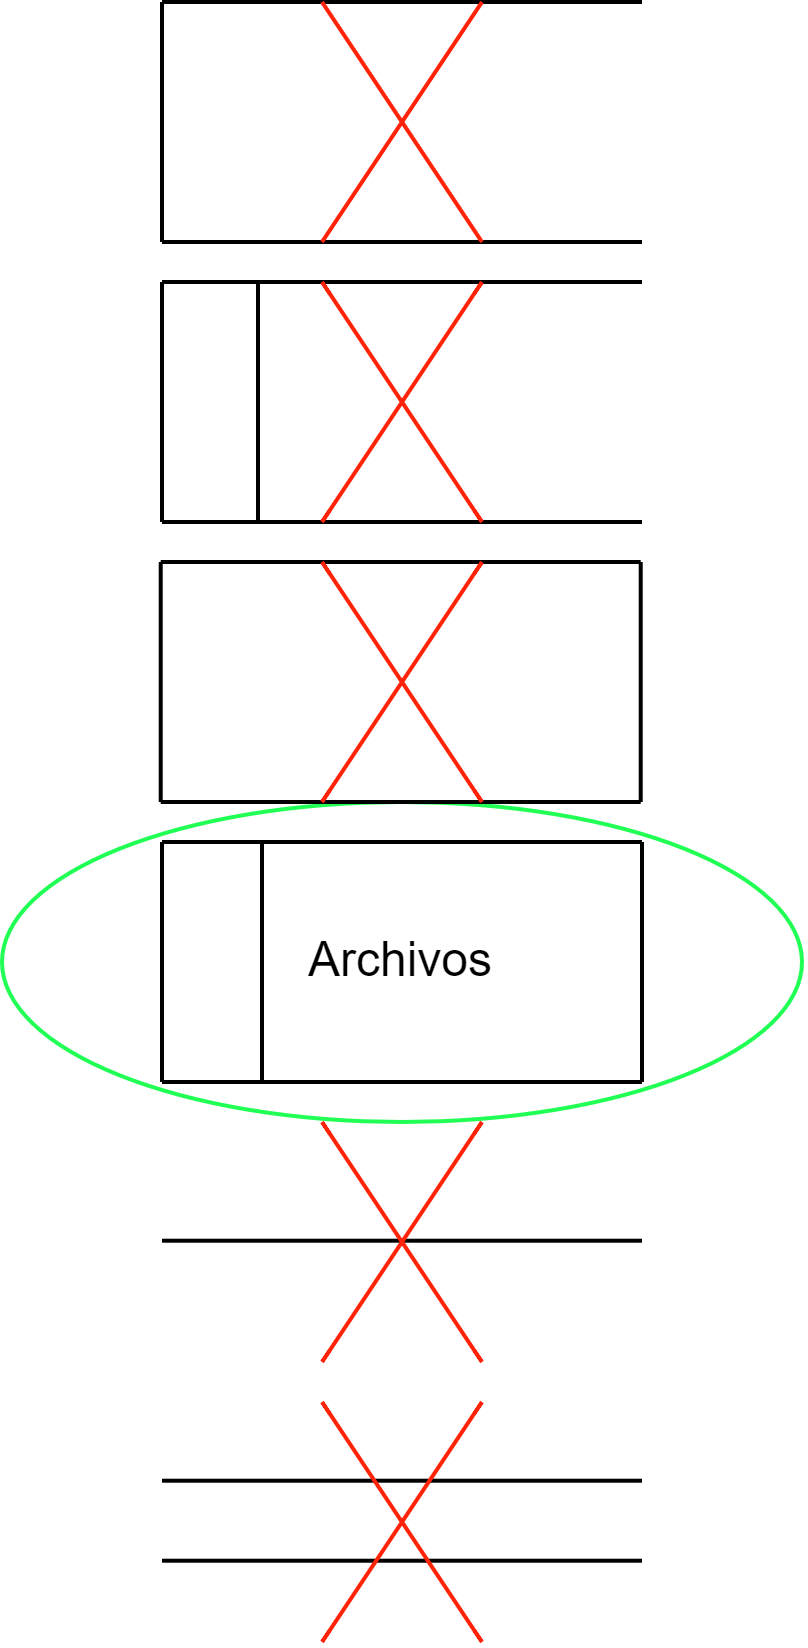
\includegraphics[width=0.80\textwidth]{img/archivos.png}
\end{figure}
\newpage
\subsection{Características generales de los elementos de un DFD}
\noindent\textbf{Entidades:} Son los elementos que generan o consumen información.
\begin{itemize}
    \item No existen relaciones (flujos) entre entidades.
    \item Se pueden repetir entidades colocando una linea diagonal en la esquina superior derecha por cada copia.
\end{itemize}
\textbf{Procesos:} Son las actividades que se realizan sobre la información.
\begin{itemize}
    \item Nombres de los procesos terminan en verbo o en -ción.
\end{itemize}
\textbf{Flujos:} Son las flechas que indican el movimiento de la información.
\begin{itemize}
    \item Nombre de los flujos \textbf{NO} terminan por verbo \\(Ej.: Apunte entregado $\rightarrow$ Entregar apunte).
    \item Nombres de flujos de archivos en formato: ``información.requerida-nombre.archivo''.
    \item Nombre de flujos no se pueden repetir.
    \item Elementos son flujos de datos.
    \item Lineas de flujo no se cruzan.
    \item No son acciones.
    \item Evitar redundancias.
\end{itemize}
\textbf{Archivos:} Son los almacenes de información.
\begin{itemize}
    \item Archivos se relacionan con procesos y no con entidades
    \item Archivos no se relacionan entre si.
\end{itemize}
\subsubsection{Identificación de entidades}
\begin{enumerate}
    \item Todo aquel que aporte algún dato al proceso y que no forme parte del proceso es entidad.
    \item Todo aquel que reciba información del proceso y que no forme parte del proceso es entidad.
    \item Todo aquel que lleve a cabo el proceso, que este a cargo del proceso y/o forma parte del proceso, no es entidad.
\end{enumerate}
\end{document}
